\documentclass[12 pt]{article}
\usepackage[utf8]{inputenc}
\usepackage[T1]{fontenc}
\usepackage[spanish, es-tabla]{babel}
\usepackage[margin=1.8cm]{geometry}
\usepackage{graphicx}
\usepackage{longtable}
\usepackage{wrapfig}
\usepackage{rotating}
\usepackage[normalem]{ulem}
\usepackage{amsmath}
\usepackage{amssymb}
\usepackage{amsthm}
\usepackage{capt-of}
\usepackage{hyperref}
\usepackage{float}
\hypersetup{
  colorlinks=true,
  linkcolor=blue,
  filecolor=magenta,      
  urlcolor=cyan,
  pdfauthor={Victor Federico Torres Trejo},
  pdftitle={Informe Final de Servicio Social},
  pdfkeywords={},
  pdfsubject={},
  pdfcreator={Victor Torres}, 
  pdflang={Spanish}
}

\usepackage[export]{adjustbox}
\usepackage{caption}
\usepackage{subcaption}
\usepackage{fancyhdr}
\setlength{\headheight}{14.5pt}
\pagestyle{fancy}
\fancyhf{}
\fancyhead[L]{Informe Final de Servicio Social}
\fancyhead[R]{Víctor F. Torres Trejo}
\fancyfoot[C]{\thepage}

\title{Informe Final de Servicio Social}
\author{Victor Federico Torres Trejo}

\begin{document}
\thispagestyle{empty}
\begin{figure}[ht]
  \minipage{0.5\textwidth}
  
\includegraphics[width=4.5cm, keepaspectratio]{imagenes/Logo_UNAM.png}
  \label{EscudoUNAM}
  \endminipage
  \minipage{0.5\textwidth}
  \raggedleft
  
\includegraphics[width=4.0cm, keepaspectratio]{imagenes/Logo_FC.png}
  \label{EscudoFC}
  \endminipage
\end{figure}

\begin{center}
  \vspace{0.5cm}
  \LARGE
  UNIVERSIDAD NACIONAL AUTÓNOMA DE MÉXICO 
  
  \vspace{0.8cm}
  \LARGE
  FACULTAD DE CIENCIAS
  
  \vspace{1.0cm}	
  \Large
  \textbf{Informe Final de Servicio Social}

  \vspace{0.8cm}
  \large
  \textbf{Desarrollo de Material Didáctico y Simuladores Interactivos para Estructuras de Datos y Algoritmos}

  \vspace{0.8cm}
  \normalsize	
  Prestador \\
  \vspace{.3cm}
  \large
  \textbf{Víctor Federico Torres Trejo \\ No. de Cuenta: 422090690}
  
  \vspace{0.7cm}
  \normalsize	
  PROFESOR RESPONSABLE \\
  \vspace{.3cm}
  \large
  \textbf{Pedro Ulises Cervantes González}\\  
  \normalsize	
  \vspace{0.8cm}
  \normalsize	
  PROGRAMA \\
  \vspace{.3cm}
  \large
  \end{center}
\clearpage 

\tableofcontents
\clearpage

\section*{Ficha de Identificación del Proyecto}
\addcontentsline{toc}{section}{Ficha de Identificación del Proyecto}

\begin{table}[H]
\centering
\begin{tabular}{|p{5.5cm}|p{11.0cm}|}
\hline
\textbf{Campo} & \textbf{Detalles del Registro Académico} \\ \hline
\textbf{Alumno:} & Víctor Federico Torres Trejo \\ \hline
\textbf{No. de Cuenta:} & 422090690 \\ \hline
\textbf{Licenciatura:} & Ciencias de la Computación \\ \hline
\textbf{Institución / Facultad:} & Facultad de Ciencias, Universidad Nacional Autónoma de México \\ \hline
\textbf{Programa de Servicio Social:} & Apoyo al Personal Docente mediante la Elaboración de Material Didáctico \\ \hline
\textbf{Profesor Responsable:} & Pedro Ulises Cervantes González \\ \hline
\textbf{Periodo de Realización:} & 28 de Noviembre de 2025 – 15 de Junio de 2026 \\ \hline
\textbf{Horas Totales Reportadas:} & 480 Horas \\ \hline
\textbf{Repositorio Digital:} & \url{https://github.com/vector2202/estructuras-datos-fciencias} \\ \hline
\end{tabular}
\end{table}

\clearpage

\section*{1. Resumen Ejecutivo / Abstract}
\addcontentsline{toc}{section}{1. Resumen Ejecutivo / Abstract}

El estudio de las estructuras de datos y los distintos algoritmos tanto de las estructuras de datos como de otro estilo como ordenamiento, búsqueda, representan una parte fundamental en la formación de cualquier estudiante de Ciencias de la Computación. Aún así el pasar de los conceptos matemáticos abstractos como lo es un TDA, complejidades asintóticas, balanceo de árboles, a una implementación ya práctica suele ser una barrera muy fuerte para el estudiante universitario, puesto que hay conceptos que dificultan esta implementación de la teoría a la práctica.

Este proyecto de Servicio Social consiste en el diseño, desarrollo e integración de una serie de recursos didácticos, de código abierto. A través de distintos ejes desarrollados a lo largo de este proyecto, los cuales consisten en apuntes teóricos rigurosos, ejercicios prácticos programados en \texttt{Java} el cual es el lenguaje de programación usado a lo largo de la materia de estructuras de datos en la Facultad de Ciencias, bajo un robusto motor de compilación llamado \texttt{Bazel} el cual es desarrollado y utilizado por Google, y por último simuladores web dinámicos desarrollados con tecnologías puras (\texttt{HTML5/CSS3/JS}) se estructuró un repositorio de libre acceso para apoyar al personal docente de la facultad de ciencias de la UNAM. El proyecto se completó conforme al cronograma establecido inicial de 480 horas, entregando un repositorio educativo interactivo, con tecnologías modernas y de código abierto y libre acceso para la comunidad académica.

\section*{2. Introducción y Justificación Académica}
\addcontentsline{toc}{section}{2. Introducción y Justificación Académica}

En el estudio de las ciencias de la computación, a menudo, la teoría y la práctica suelen sufrir una brecha constante generada por la gran abstracción de los conceptos matemáticos que a la hora de la implementación no resultan ser tan claros como lo es en la teoría. Los textos académicos por lo regular abordan estas estructuras de datos con un alto nivel de abstracción matemática, mientras que en las prácticas realizadas en los laboratorios es más implementación técnica y funcionalidad del código.

Este proyecto se justifica por la necesidad de contar con herramientas didácticas modernas, que ayuden al aprendizaje activo del alumno. El poder visualizar cómo se restructuran los punteros ante cualquier modificación en las distintas estructuras de datos, cómo se rotan los árboles balanceados al ser modificados, cómo se dividen las llamadas a los algoritmos recursivos, todo esto ayuda a que los ayudantes pasen de la intuición algorítmica a la implementación formal de las estructuras de datos y sus algoritmos de una manera más sencilla y sin tantas complicaciones.

Al estructurar todos estos recursos en este repositorio, se busca ayudar al docente con herramientas visuales robustas para sesiones síncronas de clases, y se busca ayudar a los alumnos con trabajo asíncrono con los ejercicios, que al incluir pruebas unitarias se busca que ellos no dependan de un profesor que verifique su solución.

\section*{3. Objetivos del Proyecto}
\addcontentsline{toc}{section}{3. Objetivos del Proyecto}

\subsection*{3.1 Objetivo General}
\addcontentsline{toc}{subsection}{3.1 Objetivo General}

El objetivo de este proyecto de servicio social es el apoyar a los docentes de la Facultad de Ciencias de la UNAM con recursos didácticos modernos para la unidad de aprendizaje de estructuras de datos y algoritmos. Esto mediante la elaboración de material teórico riguroso, simuladores interactivos de código abierto, fortaleciendo así el proceso de aprendizaje en temas claves de algoritmos, análisis de complejidad y estructuras de datos.

\subsection*{3.2 Objetivos Específicos}
\addcontentsline{toc}{subsection}{3.2 Objetivos Específicos}
\begin{enumerate}
    \item \textbf{Investigar y Diseñar:} Analizar el plan de estudio de la unidad de aprendizaje de estructura de datos para definir los temas prioritarios y definir los requerimientos a cubrir.
    \item \textbf{Desarrollar Contenido Teórico:} Escribir notas teóricas estructuradas con definiciones formales, con ejemplos claros y casos de uso.
    \item \textbf{Programar Simuladores Interactivos:} Diseñar y crear simuladores visuales dinámicos basados en tecnologías web, que permitan interactuar con la lógica de las estructuras de datos sin necesidad de configuraciones previas complejas.
    \item \textbf{Construir Laboratorios Prácticos:} Diseñar e implementar ejercicios de programación en Java, utilizando un sistema de construcción industrial como Bazel para asegurar la reproducibilidad y el testing automatizado de las soluciones de los estudiantes.
    \item \textbf{Consolidar e Integrar:} Estructurar el repositorio de manera ordenada y documentada.
\end{enumerate}

\section*{4. Marco Referencial}
\addcontentsline{toc}{section}{4. Marco Referencial}

El enseñar estructuras de datos y algoritmos a nivel universitario representa un reto único, ya que requiere que el alumno comprenda conceptos abstractos y matemáticos, los lleve a la implementación y la comprensión de estos temas determinará en gran parte la comprensión de otras unidades de aprendizaje. Es decir alumnos que tengan una buena base de estructura de datos se desempeñarán de mejor manera en unidades posteriores de la licenciatura. Es por ello que clases teóricas a veces necesitan de apoyo práctico y visual. Algunos temas que se observa que representan un reto para los alumnos son:

\begin{itemize}
    \item \textbf{Invisibilidad de la Memoria Dinámica:} La asignación y liberación de memoria física, la manipulación de referencias y el comportamiento del recolector de basura son conceptos abstractos difíciles de mentalizar. Los alumnos suelen cometer errores lógicos debido a la falta de un modelo mental claro de la memoria.
    \item \textbf{Retroalimentación Asíncrona Deficiente:} En los laboratorios de la facultad, los estudiantes escriben soluciones de código y deben esperar a que se les proporcione retroalimentación formal. Sin pruebas unitarias locales, los estudiantes carecen de una retroalimentación inmediata sobre la correctitud de su código en casos que suelen romper el código y el alumno suele tardar en identificar.
\end{itemize}

La integración de \textbf{visualizadores interactivos en tiempo real} y \textbf{ejercicios con pruebas unitarias locales} ayuda a resolver estos retos. La interacción con un simulador interactivo ayuda a comprender los enlaces y punteros y operaciones estructurales necesarias. Mientras que un entorno como Bazel, provee la retroalimentación con solo correr un comando.

\section*{5. Arquitectura del Proyecto}
\addcontentsline{toc}{section}{5. Arquitectura del Proyecto}

Se propuso la siguiente arquitectura de desarrollo basada en tres distintas secciones:

\subsection*{5.1 Eje Teórico}
\addcontentsline{toc}{subsection}{5.1 Eje Teórico}
La documentación teórica no debe depender de qué editor o lector de textos se utilice. Se usó \texttt{org-mode} (Emacs) debido a su excelente manejo de texto plano estructurado, su capacidad nativa para integrar bloques de código interactivos y su perfecta conversión a sistemas tipográficos científicos con \texttt{\LaTeX}. Esto permite una flexibilidad de generar a partir de estos archivos distintos archivos (pdf, latex, html) según se requiera.

\subsection*{5.2 Eje Visual}
\addcontentsline{toc}{subsection}{5.2 Eje Visual}

El desarrollo de los simuladores visuales se hizo basándose en las tecnologías web (HTML5, CSS3 y JavaScript). Se buscó evitar el uso de frameworks pesados (como React, Angular o Vue).
\begin{itemize}
    \item \textbf{Justificación Técnica:} Los proyectos basados en frameworks web modernos requieren un proceso de construcción y mantenimiento complejo, y debido a que el propósito de este proyecto es facilitar el uso e instalación al estudiante, se evitó su uso. Al utilizar tecnologías nativas del navegador, se asegura que los simuladores puedan ejecutarse en cualquier sistema solamente abriendo el archivo \texttt{index.html} en el navegador, o levantando un servidor web básico con \texttt{python3 -m http.server}. Esto garantiza un uso simple para el estudiante y durabilidad del material.
\end{itemize}

\subsection*{5.3 Eje Práctico}
\addcontentsline{toc}{subsection}{5.3 Eje Práctico}
Para el desarrollo y evaluación del código práctico se eligió \textbf{Java}, debido a que es el lenguaje utilizado por la unidad de aprendizaje. Java permite la manipulación de referencias, lo que es muy importante para la comprensión de las estructuras de datos. Para eliminar los problemas comunes de classpath e incompatibilidades de compilación en las distintas máquinas de los estudiantes, se integró \textbf{Google Bazel}.
\begin{itemize}
    \item \textbf{Justificación Técnica:} Bazel proporciona una compilación hermética y reproducible mediante la especificación explícita de entradas y salidas en archivos \texttt{BUILD}. El uso de pruebas unitarias parametrizadas con JUnit permite una metodología de auto-evaluación donde el docente proporciona esqueletos de código (\texttt{// TODO}) y el estudiante valida su implementación local de forma determinista mediante el comando \texttt{bazel test //...}. Adicionalmente se considera que el uso de estas tecnologías pueden beneficiar al alumno a familiarizarse con herramientas profesionales de la industria.
\end{itemize}

\section*{6. Desarrollo Cronológico de Actividades}
\addcontentsline{toc}{section}{6. Desarrollo Cronológico de Actividades}

A continuación, se presenta el informe cronológico de las actividades ejecutadas durante la prestación del Servicio Social:

\subsection*{Fase 1: Planeación General, Investigación y Diseño de Estructura (28 nov – 31 dic 2025)}
\addcontentsline{toc}{subsection}{Fase 1: Planeación General, Investigación y Diseño de Estructura (28 nov – 31 dic 2025)}
\begin{itemize}
    \item \textbf{Actividades Ejecutadas:}
    \begin{itemize}
        \item Análisis del plan de estudios y material disponible de la unidad de aprendizaje de Estructuras de Datos y Algoritmos.
        \item Definición de la estructura de directorios del repositorio git y selección del stack tecnológico.
        \item Planteamiento del flujo de trabajo hermético para Java (configuración de Bazel en la raíz del proyecto).
    \end{itemize}
    \item \textbf{Entregables:} Estructura inicial del repositorio organizada en carpetas (\texttt{/notas}, \texttt{/ejercicios}, \texttt{/proyectos}, \texttt{/docs}), y archivos de configuración del espacio de trabajo base \texttt{MODULE.bazel}, \texttt{.gitignore} y el \texttt{README.md} de bienvenida y especificaciones del proyecto.
\end{itemize}

Durante este periodo inicial, el reto principal consistió en concebir un esquema de archivos que fuera intuitivo para alumnos novatos pero técnicamente riguroso. Se optó por una división limpia de tres áreas fundamentales: teoría (\texttt{/notas}), práctica dirigida (\texttt{/ejercicios}) y visualización interactiva (\texttt{/proyectos}). La planeación incluyó la investigación profunda sobre sistemas de construcción, eligiendo a Bazel por su habilidad para descargar y cachear herramientas de compilación de forma transparente, aislando al estudiante de tener que instalar compiladores JDK específicos de manera local.

\subsection*{Fase 2: Desarrollo del Material de Estructuras Lineales (1 ene – 31 ene 2026)}
\addcontentsline{toc}{subsection}{Fase 2: Desarrollo del Material de Estructuras Lineales (1 ene – 31 ene 2026)}
\begin{itemize}
    \item \textbf{Actividades Ejecutadas:}
    \begin{itemize}
        \item Redacción de apuntes teóricos detallados sobre estructuras de datos lineales las cuales son: Arreglos, Listas (simplemente ligadas, doblemente ligadas, circulares), Pilas y Colas.
        \item Programación de los esqueletos de código en Java y definición de baterías de pruebas unitarias robustas en \texttt{/ejercicios} para cada estructura lineal.
    \end{itemize}
    \item \textbf{Entregables:} 
    \begin{itemize}
        \item Notas académicas en Org-mode para la introducción a la complejidad y estructuras lineales en \texttt{/notas/01\_complejidad\_algoritmica}, \texttt{/notas/02\_tda}, \texttt{/notas/03\_arreglos}, \texttt{/notas/04\_listas/notas.org}, \texttt{/notas/05\_pilas} y \texttt{/notas/06\_colas}.
        \item Laboratorios prácticos programados en Java con aserciones JUnit listas para autoevaluación en \texttt{/ejercicios/listas/}, \texttt{/ejercicios/pilas/} y \texttt{/ejercicios/colas/} junto con sus respectivos archivos de compilación \texttt{BUILD}.
    \end{itemize}
\end{itemize}

En esta fase, los conceptos teóricos desarrollados fueron centrados en detallar los costos temporales de operaciones elementales. Para los ejercicios hechos en java se diseñaron pruebas unitarias usando JUnit cubriendo incluso casos extremos, forzando así al alumno a programar con robustez sus soluciones.

\subsection*{Fase 3: Diseño y Programación de Simuladores Lineales (1 feb – 29 feb 2026)}
\addcontentsline{toc}{subsection}{Fase 3: Diseño y Programación de Simuladores Lineales (1 feb – 29 feb 2026)}
\begin{itemize}
    \item \textbf{Actividades Ejecutadas:}
    \begin{itemize}
        \item Diseño visual e implementación interactiva con JavaScript del visualizador de Listas y Arreglos dinámicos permitiendo operaciones dinámicas con animaciones CSS.
        \item Creación de simuladores FIFO/LIFO dinámicos para representar el comportamiento de Pilas y Colas.
        \item Integración de una base de estilos global (\texttt{global.css}) para dotar de una identidad visual premium y unificada a todos los simuladores.
    \end{itemize}
    \item \textbf{Entregables:}
    \begin{itemize}
        \item Simuladores web operacionales en \texttt{/proyectos/03\_arreglos} (Simulador de Arreglos dinámicos), \texttt{/proyectos/04\_listas} (Lista Doblemente Enlazada animada), \texttt{/proyectos/05\_pilas} (Simulador de Pila) y \texttt{/proyectos/06\_colas} (Simulador de Cola).
        \item Carpeta de demostración rápida en \texttt{/proyectos/ejemplos\_estructuras\_lineales} y el sistema de diseño centralizado e identidades CSS visuales en \texttt{/proyectos/global.css} y \texttt{/proyectos/styles.css}.
    \end{itemize}
\end{itemize}

El reto técnico más grande de esta fase fue sincronizar las animaciones del frontend con el estado interno de la estructura. Utilizando JavaScript moderno, se implementó un motor de animación asíncrono, junto con transiciones CSS controladas por clases. Esto permitió que al dar clic en "insertar nodo", el usuario pueda ver el nacimiento físico del nodo en pantalla, la animación del recorrido del puntero temporal buscando la posición, y la re-conexión física de las flechas de enlace en tiempo real, facilitando la comprensión intuitiva de la complejidad $\mathcal{O}(N)$ frente a $\mathcal{O}(1)$.

\subsection*{Fase 4: Teoría y Práctica de Estructuras No Lineales (1 mar – 31 mar 2026)}
\addcontentsline{toc}{subsection}{Fase 4: Teoría y Práctica de Estructuras No Lineales (1 mar – 31 mar 2026)}
\begin{itemize}
    \item \textbf{Actividades Ejecutadas:}
    \begin{itemize}
        \item Redacción de las guías didácticas teóricas sobre Estructuras Jerárquicas y No Lineales: Árboles Binarios de Búsqueda (BST), Árboles Auto-balanceados (AVL, Rojinegros), Heaps, Tablas Hash y Gráficas.
        \item Diseño de ejercicios prácticos retadores para Árboles y Hash Tables en Java.
        \item Programación del simulador interactivo de Árboles y recorridos en preorden, inorden y postorden, así como simuladores de tablas hash, heaps y gráficas.
    \end{itemize}
    \item \textbf{Entregables:}
    \begin{itemize}
        \item Guías didácticas teóricas completas en \texttt{/notas/07\_arboles}, \texttt{/notas/08\_heaps}, \texttt{/notas/09\_hash} y \texttt{/notas/10\_graficas}.
        \item Simuladores web e interactivos funcionales en \texttt{/proyectos/07\_arboles} (recorrido de árboles binarios), \texttt{/proyectos/08\_heaps} (visualización de montículos), \texttt{/proyectos/09\_hash} (simulador de indexación y colisiones) y \texttt{/proyectos/10\_graficas} (visualización de nodos y conexiones de grafos).
        \item Laboratorios y pruebas unitarias complejas en \texttt{/ejercicios/arboles/}, \texttt{/ejercicios/hash/} y \texttt{/ejercicios/graficas/}.
    \end{itemize}
\end{itemize}

Al migrar a estructuras no lineales, el grado de abstracción se incrementó. Para el simulador web de árboles binarios, se implementó una representation visual autogestionada mediante un algoritmo de distribución espacial que recalcula las coordenadas $(X, Y)$ de los nodos secundarios dinámicamente al insertar o eliminar elementos. El simulador permite activar los recorridos (Preorden, Inorden, Postorden), iluminando progresivamente los nodos visitados para que el estudiante comprenda el flujo de la pila recursiva.

\subsection*{Fase 5: Algoritmos de Búsqueda, Ordenamiento y Backtracking (1 abr – 30 abr 2026)}
\addcontentsline{toc}{subsection}{Fase 5: Algoritmos de Búsqueda, Ordenamiento y Backtracking (1 abr – 30 abr 2026)}
\begin{itemize}
    \item \textbf{Actividades Ejecutadas:}
    \begin{itemize}
        \item Desarrollo de la guía teórica y ejemplos prácticos de Análisis de Complejidad Temporal (notaciones Big-O, Big-Omega, Big-Theta).
        \item Elaboración de simuladores dinámicos para visualizar algoritmos clásicos de ordenamiento (Bubble Sort, Insertion Sort, Quick Sort, Merge Sort) y algoritmos de búsqueda lineal y binaria.
        \item Creación de un simulador específico altamente pedagógico para ilustrar la técnica de \emph{Backtracking} (árboles de decisión en reversa).
    \end{itemize}
    \item \textbf{Entregables:}
    \begin{itemize}
        \item Apuntes teóricos dedicados en \texttt{/notas/11\_ordenamientos}.
        \item Simulador web de análisis en \texttt{/proyectos/01\_complejidad\_algoritmica} (visualizador interactivo de crecimiento de funciones y notación asintótica).
        \item Simulador de backtracking y árboles recursivos en \texttt{/proyectos/simulador\_backtracking/} junto con los visualizadores dinámicos integrados en el dashboard principal para algoritmos de ordenamiento lineal y binario.
        \item Laboratorios prácticos estructurados en Java en \texttt{/ejercicios/sorting/} (Quick Sort, Merge Sort, etc.) y \texttt{/ejercicios/busqueda/} (Búsqueda Binaria/Lineal).
    \end{itemize}
\end{itemize}

Esta fase se centró en la algoritmia y la eficiencia. El simulador de ordenamientos permite comparar visualmente la diferencia radical entre algoritmos cuadráticos ($\mathcal{O}(N^2)$) y logarítmicos ($\mathcal{O}(N \log N)$) controlando la velocidad de reproducción de las barras de tamaño. Adicionalmente, el simulador de \emph{Backtracking} resuelve dinámicamente problemas de ramificación y poda (como el laberinto o el problema de las N-Reinas), graficando al vuelo el árbol de llamadas de la recursión y coloreando de rojo los caminos fallidos antes de hacer un \emph{rollback} visual, materializando un concepto comúnmente complejo de asimilar.

\subsection*{Fase 6: Integración Final, Control de Calidad y Documentación (1 may – 15 jun 2026)}
\addcontentsline{toc}{subsection}{Fase 6: Integración Final, Control de Calidad y Documentación (1 may – 15 jun 2026)}
\begin{itemize}
    \item \textbf{Actividades Ejecutadas:}
    \begin{itemize}
        \item Unificación estética de todos los simuladores interactivos bajo una interfaz web global responsiva y atractiva.
        \item Auditoría completa del código del repositorio, verificando que todos los casos de prueba compilen y corran exitosamente mediante comandos globales de Bazel (\texttt{bazel test //...}).
        \item Redacción final de los manuales de usuario de las herramientas en sus respectivos archivos README y estructuración de este informe final.
    \end{itemize}
    \item \textbf{Entregables:}
    \begin{itemize}
        \item Dashboard unificado y responsivo en \texttt{/proyectos/index.html} que integra el acceso centralizado a los 11 simuladores.
        \item Limpieza absoluta de la compilación y aprobación de pruebas de cobertura en \texttt{/ejercicios/} certificada mediante la suite Bazel.
        \item Manuales e instrucciones didácticas en los READMEs de cada módulo y este documento final \texttt{/docs/informe\_final.md} completado y listo para conversión a PDF.
    \end{itemize}
\end{itemize}

Durante esta última fase, se realizó una revisión de código exhaustiva para limpiar advertencias de compilación y optimizar la accesibilidad de la página principal del proyecto así como revisar la legibilidad de los códigos. Se unificaron los estilos usando variables de CSS para soportar un modo oscuro nativo muy cómodo para el estudio nocturno de los alumnos. El éxito de la suite de pruebas unitarias ejecutadas a través de Bazel validó la integridad lógica del repositorio, entregando un producto docente listo para su implementación inmediata en el aula.

\section*{7. Resultados Obtenidos y Evidencia del Trabajo}
\addcontentsline{toc}{section}{7. Resultados Obtenidos y Evidencia del Trabajo}

El trabajo desarrollado se encuentra distribuido de manera ordenada y documentado en tres carpetas principales dentro del repositorio. A continuación se detallan los recursos entregados:

\subsection*{7.1 Catálogo de Notas Didácticas (\texttt{/notas})}
\addcontentsline{toc}{subsection}{7.1 Catálogo de Notas Didácticas (/notas)}
Se estructuró un conjunto de guías didácticas que abarcan el 100\% de los temas críticos del temario oficial:
\begin{enumerate}
    \item \texttt{01\_complejidad\_algoritmica}: Fundamento matemático y notación asintótica.
    \item \texttt{02\_tda}: Concepto teórico de Tipo de Dato Abstracto y encapsulamiento.
    \item \texttt{03\_arreglos}: Vectores estáticos y gestión física de memoria.
    \item \texttt{04\_listas}: Punteros y variantes de encadenamiento dinámico.
    \item \texttt{05\_pilas} y \texttt{06\_colas}: Restricciones estructurales LIFO/FIFO.
    \item \texttt{07\_arboles}, \texttt{08\_heaps} y \texttt{09\_hash}: Estructuras no lineales y direccionamiento.
    \item \texttt{10\_graficas} y \texttt{11\_ordenamientos}: Representaciones, recorridos (DFS/BFS) y ordenación.
\end{enumerate}

\subsection*{7.2 Catálogo de Ejercicios y Casos de Prueba (\texttt{/ejercicios})}
\addcontentsline{toc}{subsection}{7.2 Catálogo de Ejercicios y Casos de Prueba (/ejercicios)}
Ejercicios estructurados en Java con arquitectura Bazel para evaluación automatizada:
\begin{itemize}
    \item \textbf{/listas, /pilas, /colas}: Pruebas con JUnit para que los alumnos completen la lógica de inserción, borrado e iteración.
    \item \textbf{/sorting}: Laboratorios prácticos para implementar ordenamientos eficientes y de fuerza bruta y validar su corrección matemática de forma automatizada.
\end{itemize}

\subsection*{7.3 Catálogo de Simuladores Visuales (\texttt{/proyectos})}
\addcontentsline{toc}{subsection}{7.3 Catálogo de Simuladores Visuales (/proyectos)}

Las aplicaciones web interactivas fueron desarrolladas con un diseño moderno, intuitivo y unificado bajo estilos consistentes que garantizan una experiencia responsiva. A continuación, se presenta la galería de evidencias de los simuladores completamente operativos y sus respectivos casos de uso implementados para facilitar el aprendizaje de los alumnos:




\subsubsection*{A) Análisis de Complejidades Asintóticas y Costos Temporales}

\noindent \textbf{Recursos en \texttt{/proyectos/01\_complejidad\_algoritmica}:} Simulador interactivo que permite graficar y comparar las tasas de crecimiento de las funciones de complejidad temporal de algoritmos tradicionales (logarítmica, lineal, lineal-logarítmica, cuadrática, exponencial).
  
\begin{figure}[!ht]
  \centering
  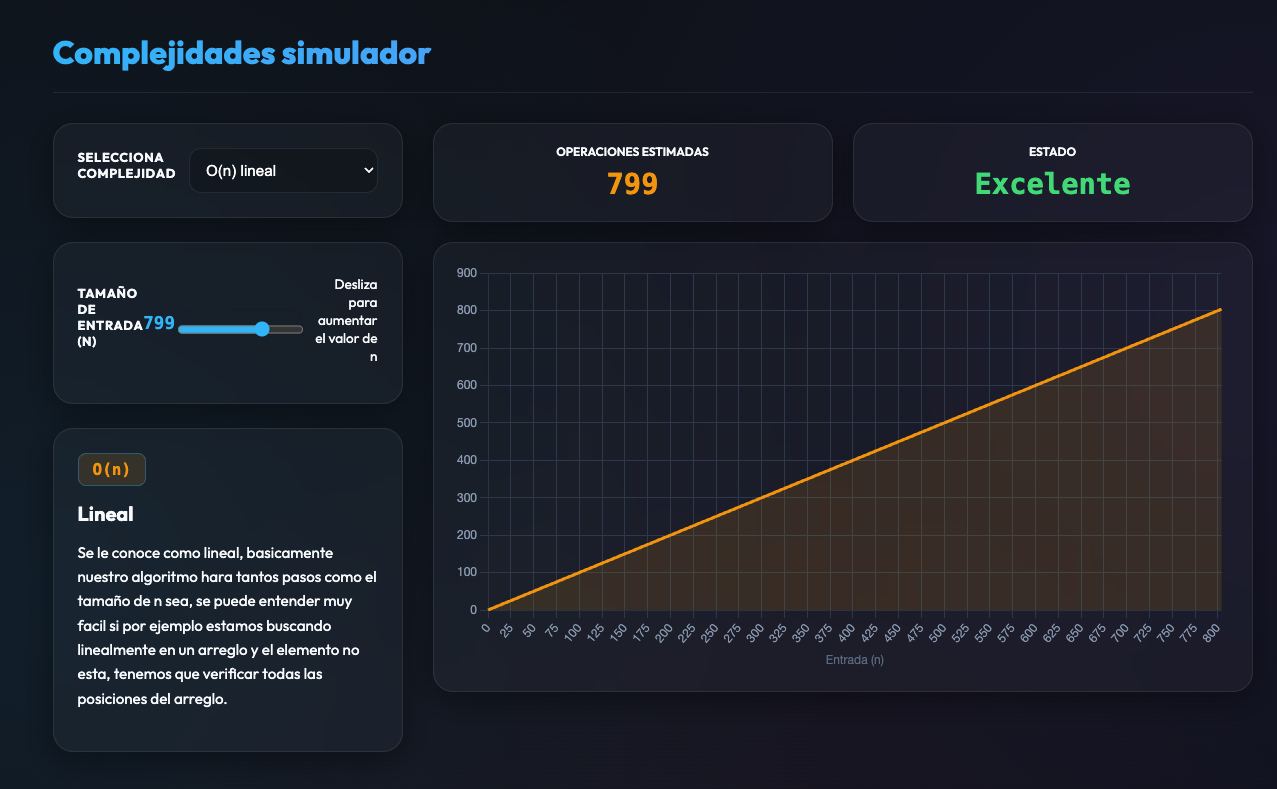
\includegraphics[width=0.85\textwidth]{imagenes/simulador_complejidades.png}
  \caption{Crecimiento de Funciones y Notación Big-O}
  \label{fig:sim_complejidades}
\end{figure}
\newpage
\begin{figure}[!ht]
  \centering
  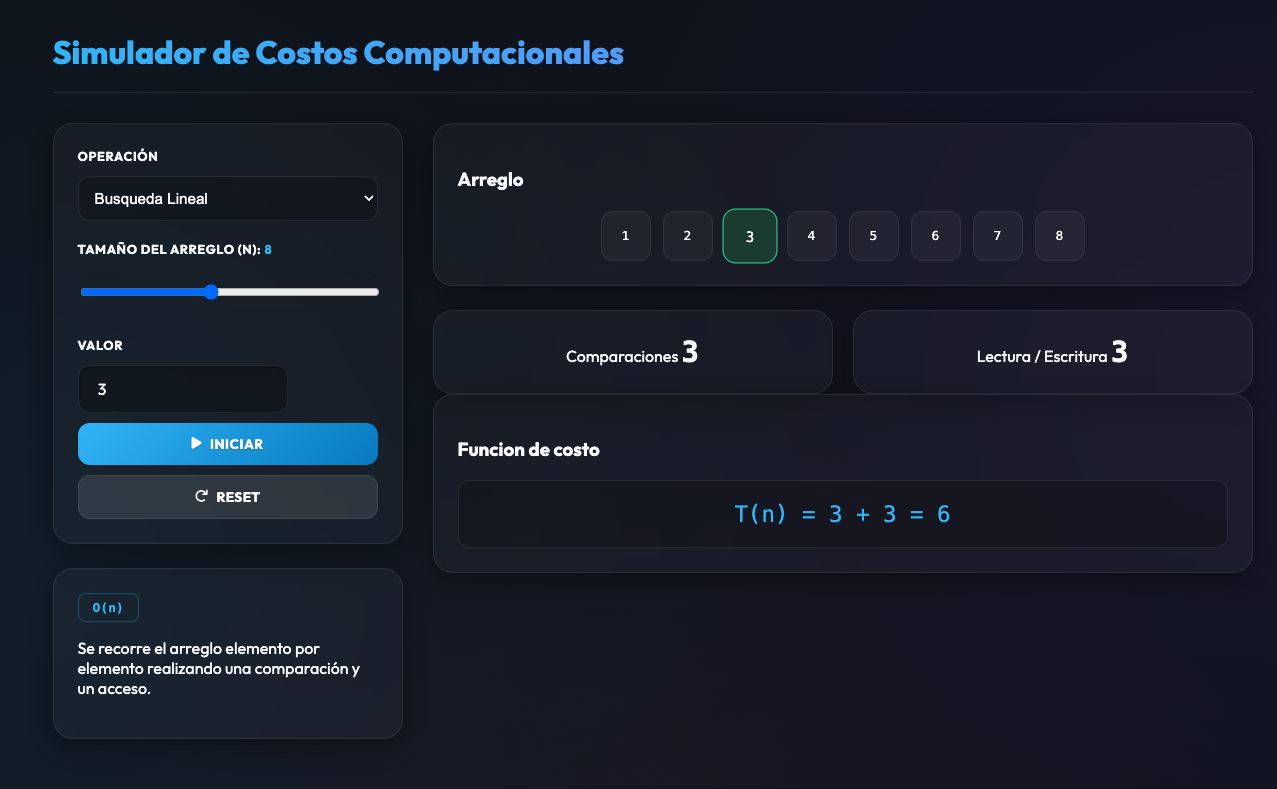
\includegraphics[width=0.85\textwidth]{imagenes/simulador_costos_comp.png}
  \caption{Tabla Comparativa de Costos Computacionales}
  \label{fig:sim_costos_comp}
\end{figure}



\subsubsection*{B) Simulador de Arreglos y Vectores Dinámicos}

\noindent \textbf{Recursos en \texttt{/proyectos/03\_arreglos}:} Visualización paso a paso de la asignación contigua de memoria, el acceso indexado en tiempo constante y el costo computacional de realizar corrimientos físicos en inserciones o eliminaciones intermedias.
\newpage
\begin{figure}[!ht]
  \centering
  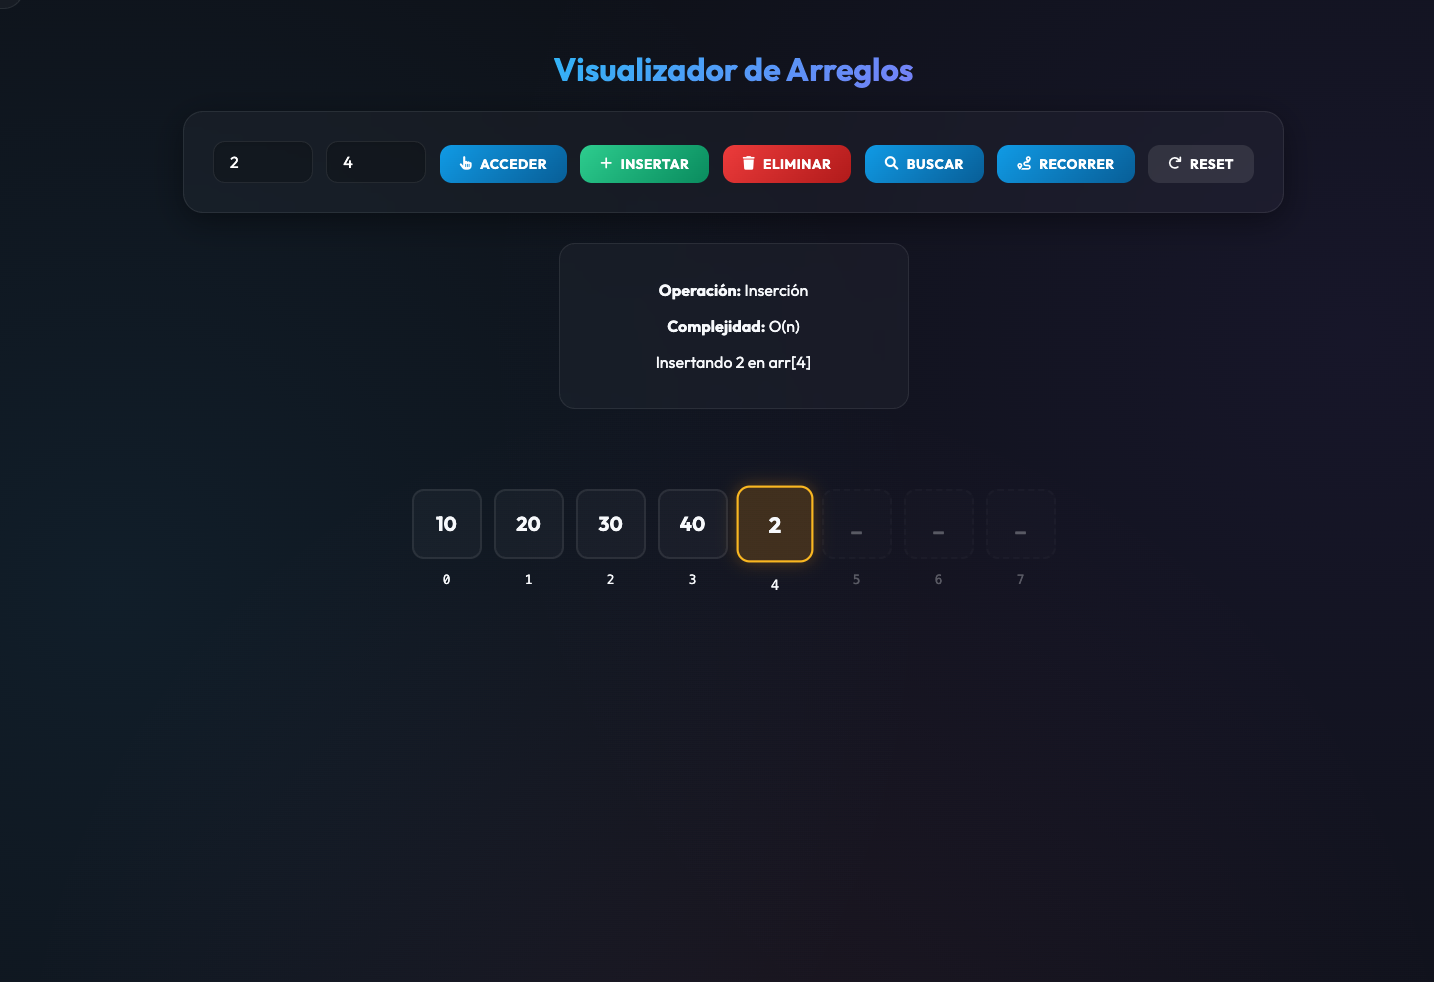
\includegraphics[width=0.85\textwidth]{imagenes/simulador_arreglos.png}
  \caption{Simulador General de Arreglos}
  \label{fig:sim_arreglos}
\end{figure}

\begin{figure}[!ht]
  \centering
  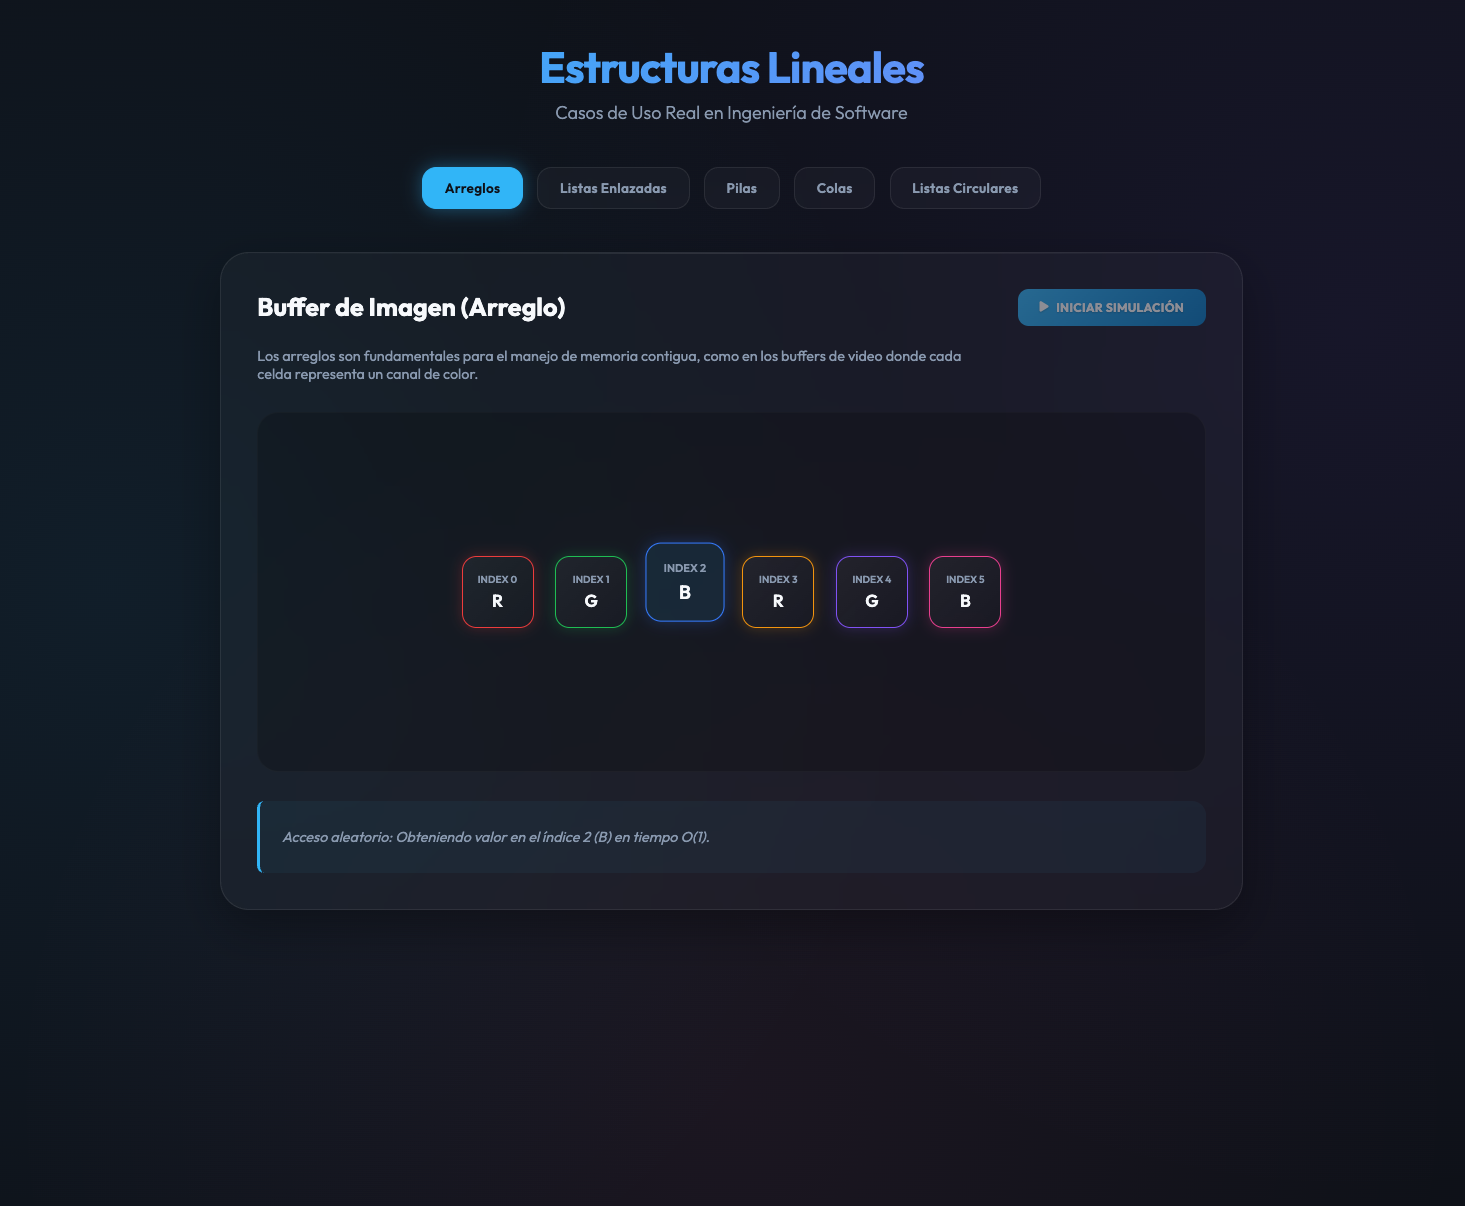
\includegraphics[width=0.85\textwidth]{imagenes/simulador_casos_uso_arreglo.png}
  \caption{Casos de Uso en Vectores Dinámicos}
  \label{fig:sim_casos_uso_arreglo}
\end{figure}
\newpage
\subsubsection*{C) Simuladores de Estructuras de Datos Lineales (Listas, Pilas y Colas)}

\noindent \textbf{Listas Enlazadas en \texttt{/proyectos/04\_listas}:} Representación animada en tiempo real de la manipulación y enlace dinámico de nodos simples, dobles y circulares.

\begin{figure}[!ht]
  \centering
  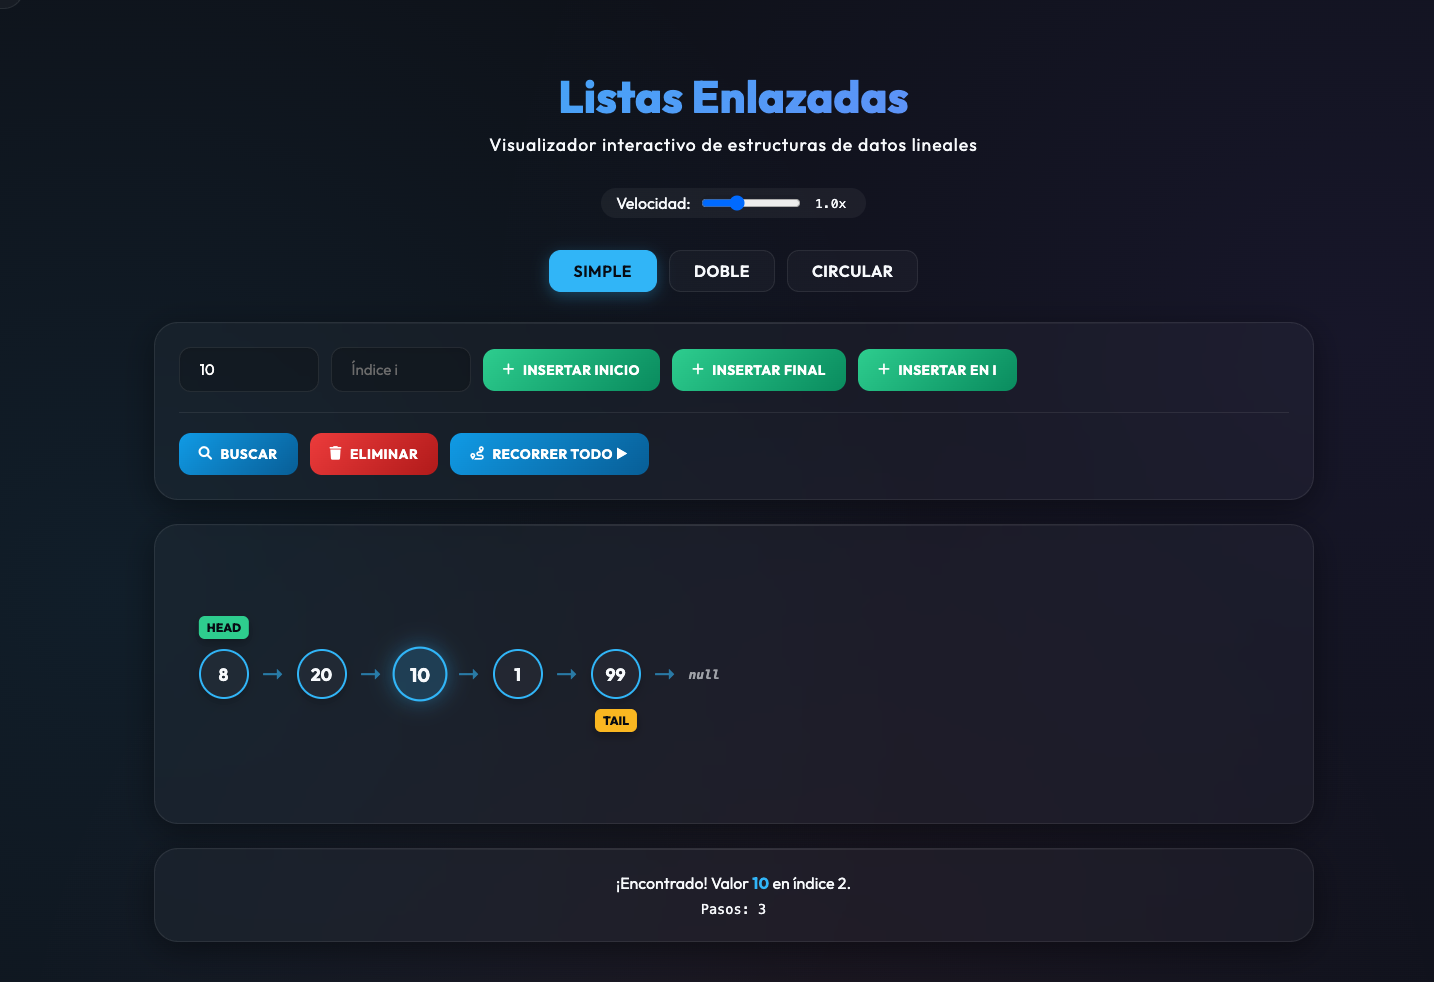
\includegraphics[width=0.85\textwidth]{imagenes/simulador_listas_simple.png}
  \caption{Simulador de Lista Simplemente Ligada}
  \label{fig:listas_simple}
\end{figure}

\begin{figure}[!ht]
  \centering
  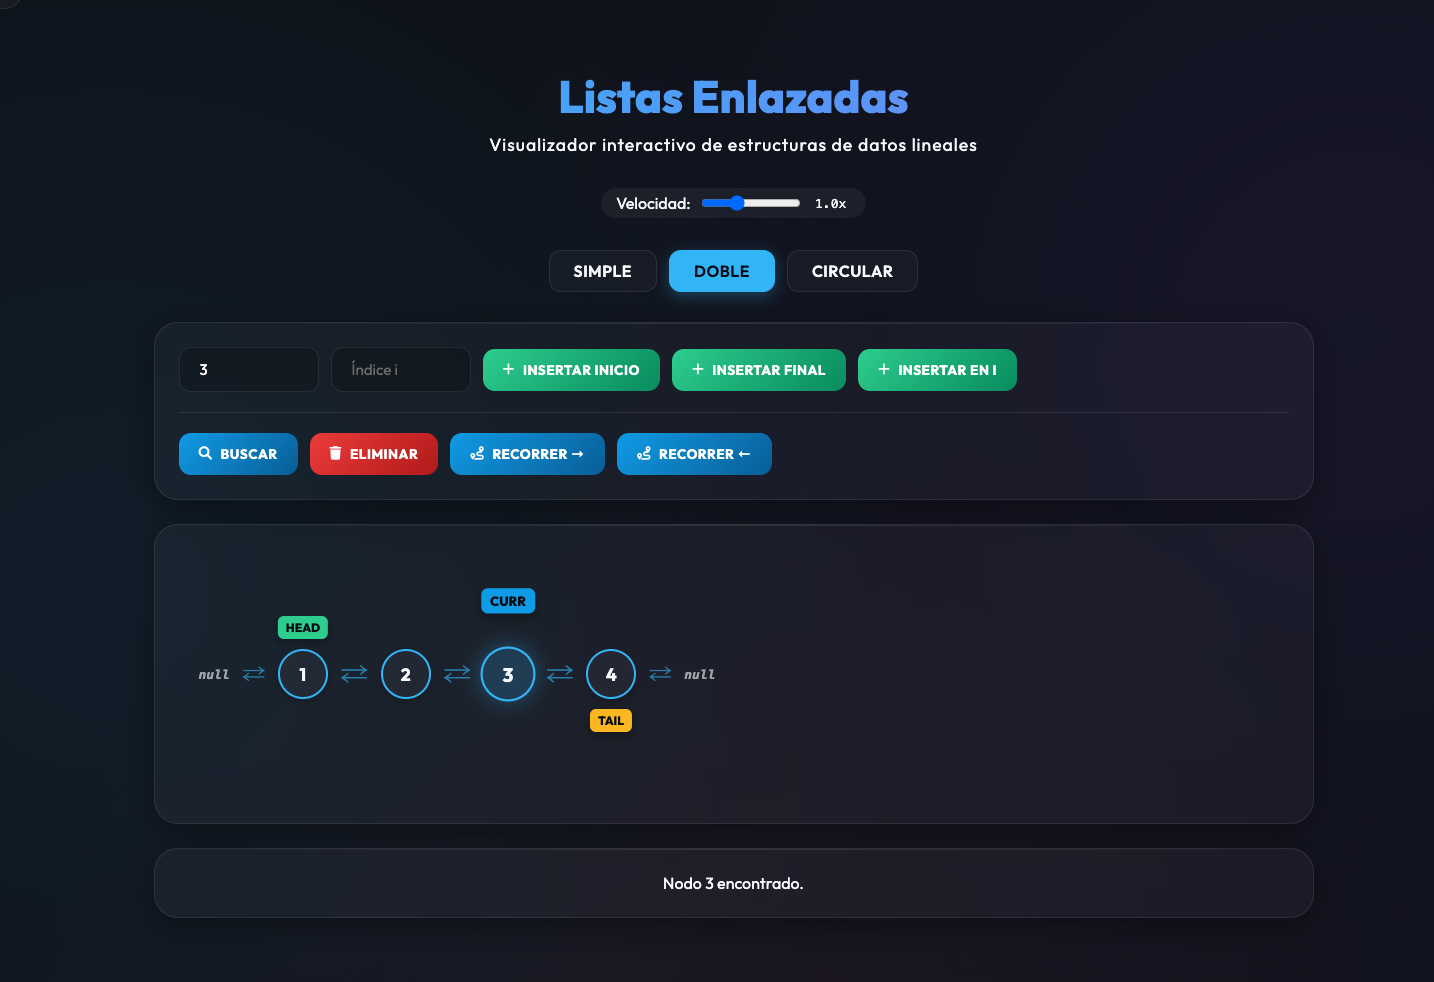
\includegraphics[width=0.85\textwidth]{imagenes/simulador_listas_doble.png}
  \caption{Simulador de Lista Doblemente Ligada}
  \label{fig:listas_doble}
\end{figure}

\newpage
\begin{figure}[!ht]
  \centering
  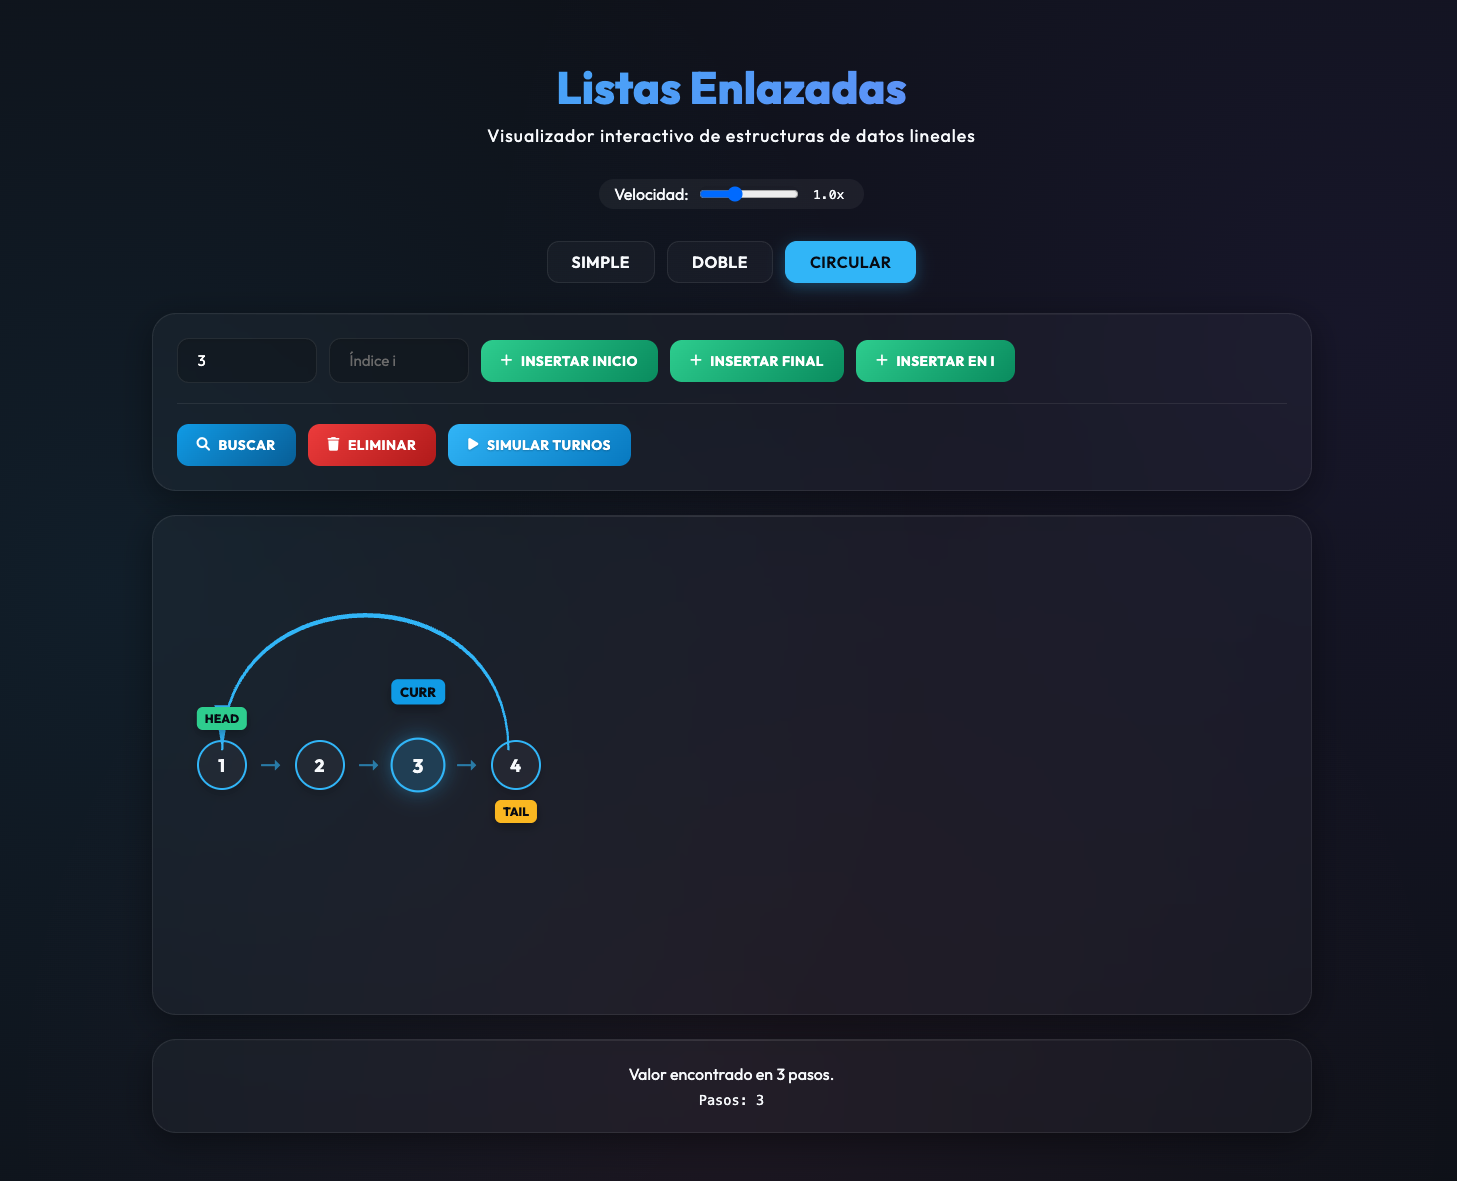
\includegraphics[width=0.88\textwidth]{imagenes/simulador_listas_circular.png}
  \caption{Simulador de Lista Circular}
  \label{fig:listas_circular}
\end{figure}


\begin{figure}[!ht]
  \centering
  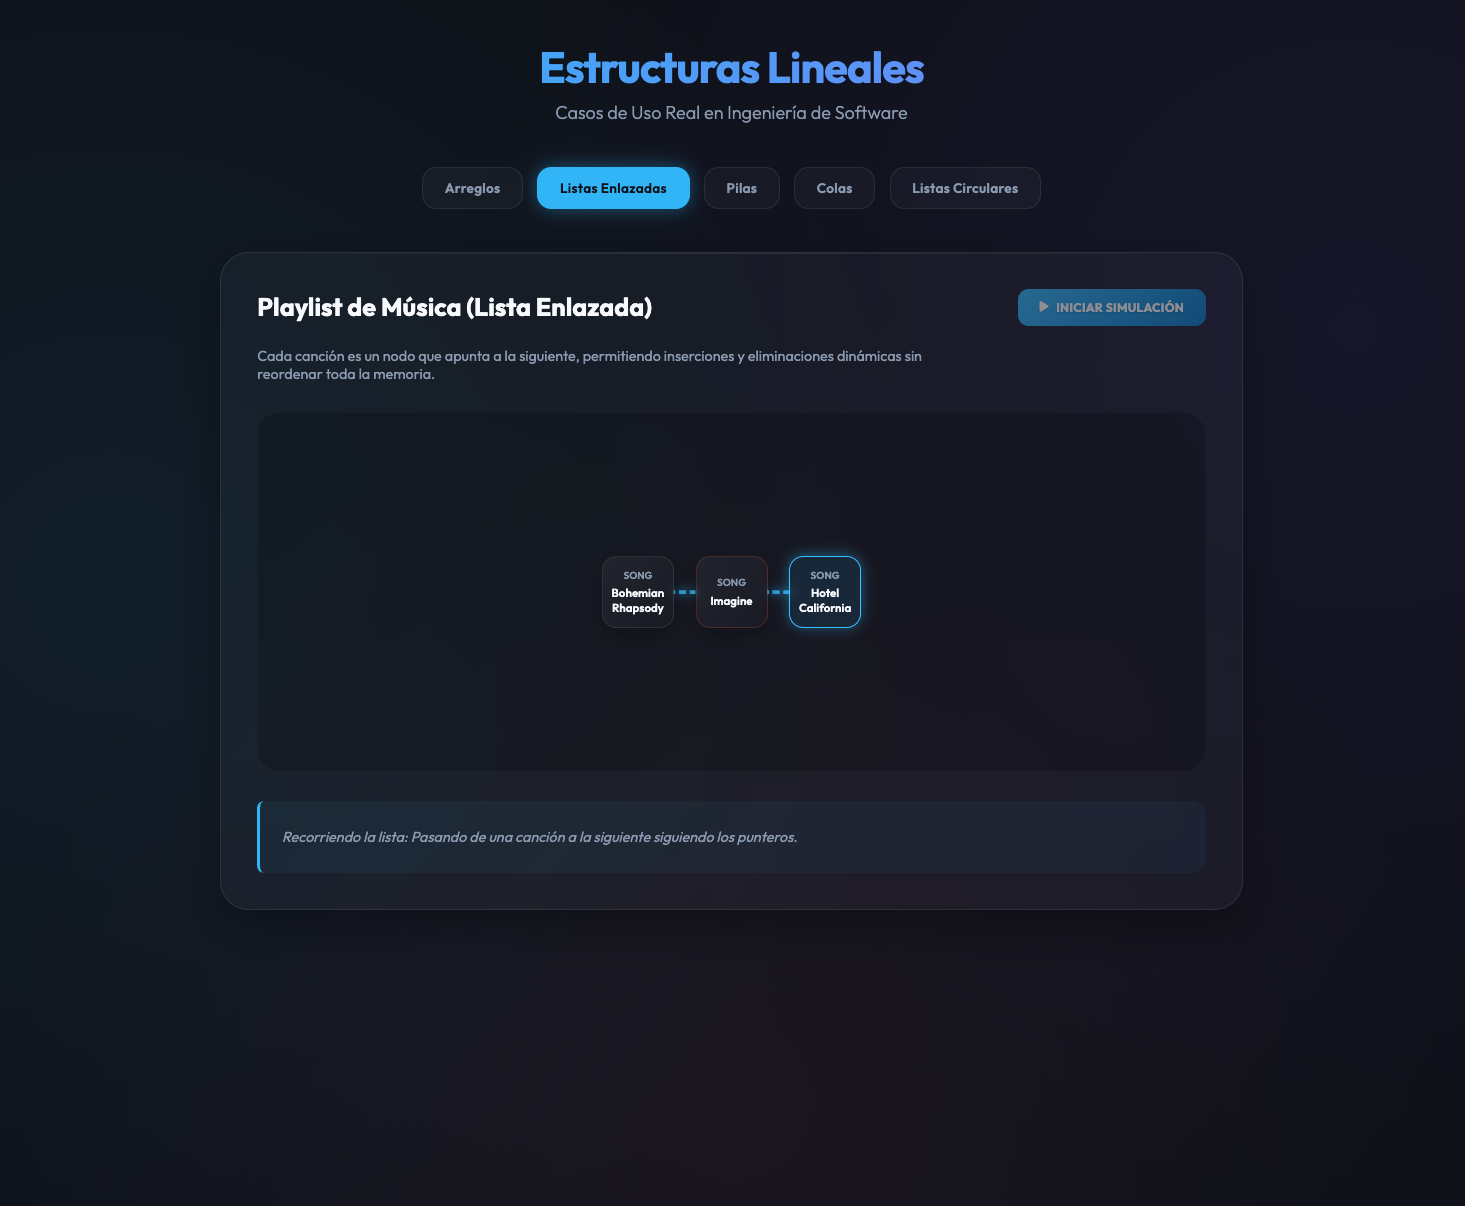
\includegraphics[width=0.85\textwidth]{imagenes/simulador_casos_uso_listas.png}
  \caption{Casos de Uso de Nodos en Listas}
  \label{fig:casos_uso_listas}
\end{figure}

\newpage

\noindent \textbf{Pilas y Colas en \texttt{/proyectos/05\_pilas} y \texttt{/proyectos/06\_colas}:} Simuladores dedicados a mostrar el comportamiento físico e interno de las políticas LIFO (\texttt{push}/\texttt{pop}) y FIFO (\texttt{enqueue}/\texttt{dequeue}), incluyendo el comportamiento circular en memoria fija.

\begin{figure}[!ht]
  \centering
  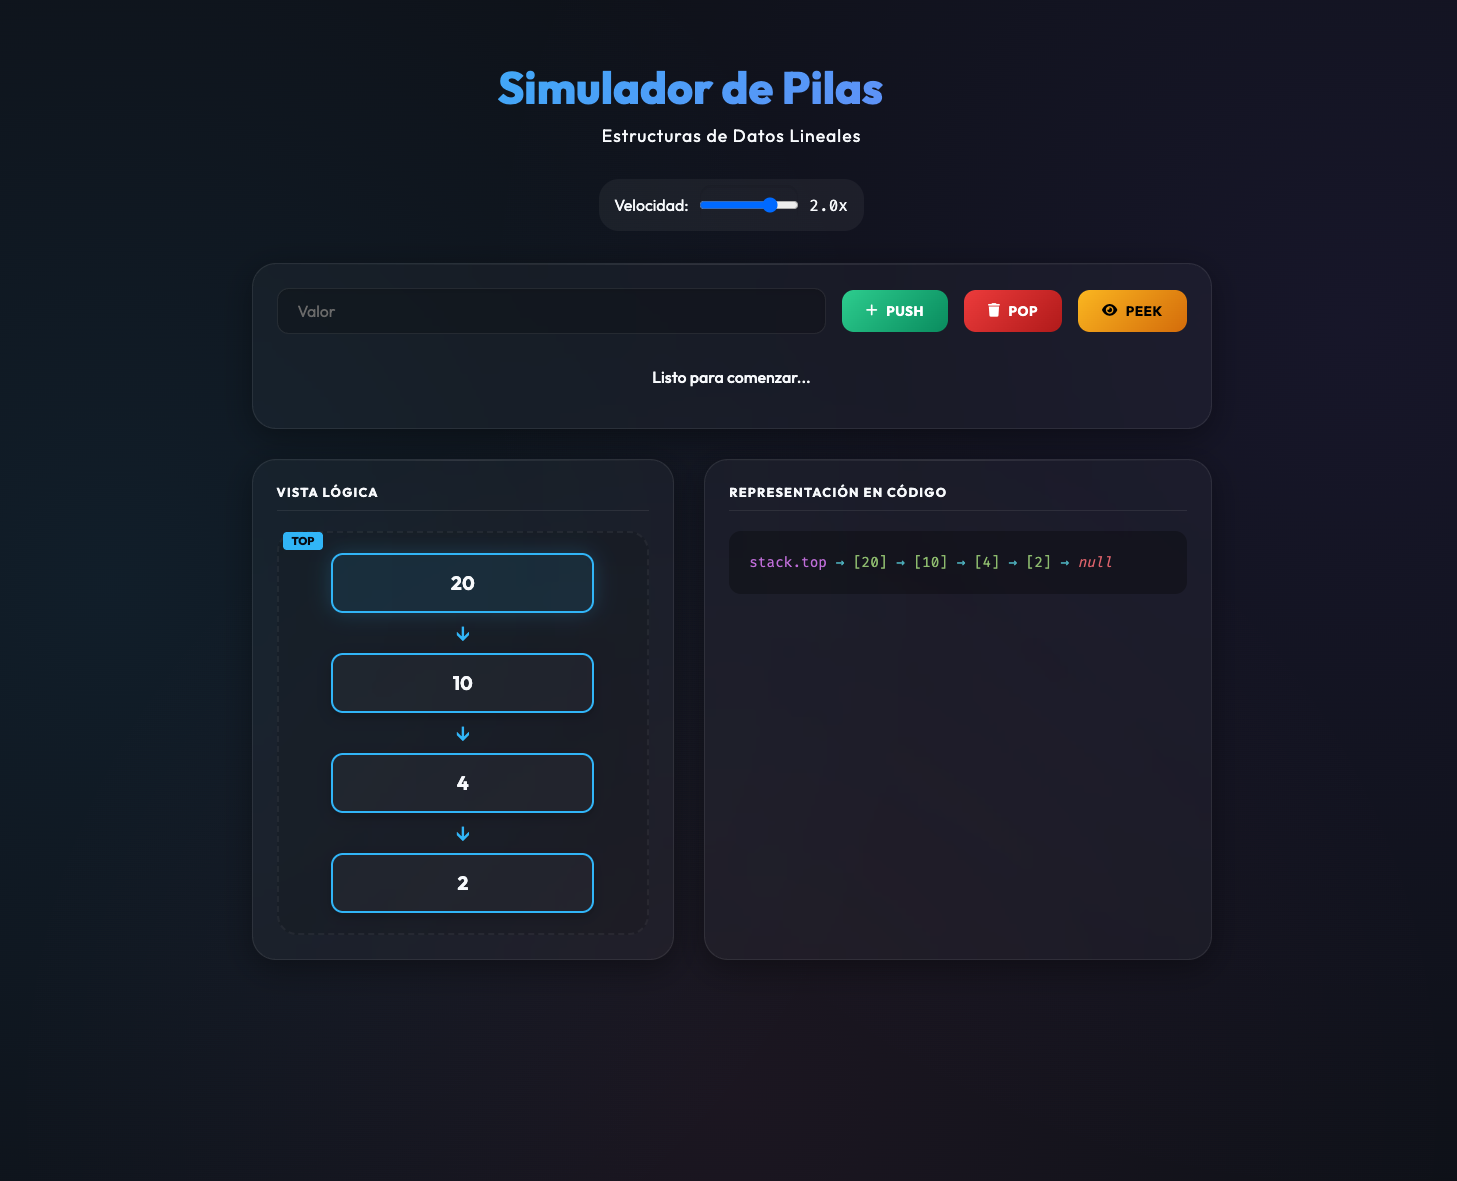
\includegraphics[width=0.85\textwidth]{imagenes/simulador_pilas.png}
  \caption{Simulador de Pilas LIFO}
  \label{fig:sim_pilas}
\end{figure}

\begin{figure}[!ht]
  \centering
  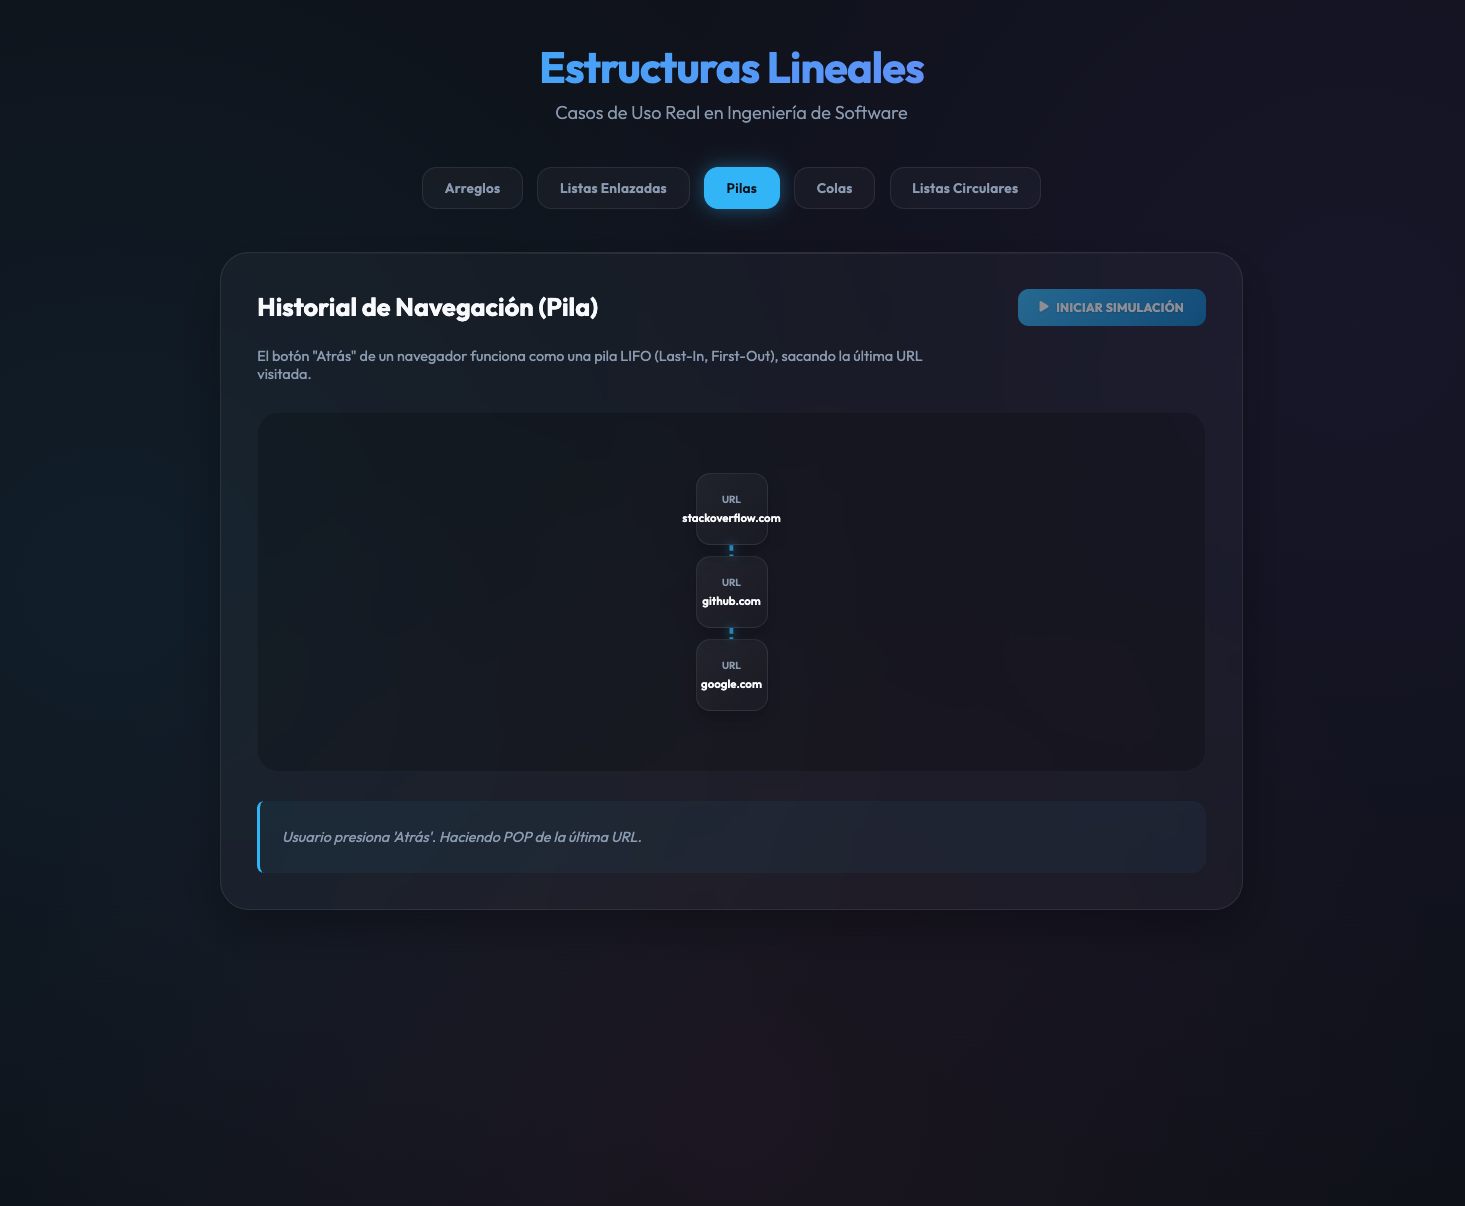
\includegraphics[width=0.85\textwidth]{imagenes/simulador_casos_uso_pilas.png}
  \caption{Casos de Uso en Pilas}
  \label{fig:casos_uso_pilas}
\end{figure}

\begin{figure}[!ht]
  \centering
  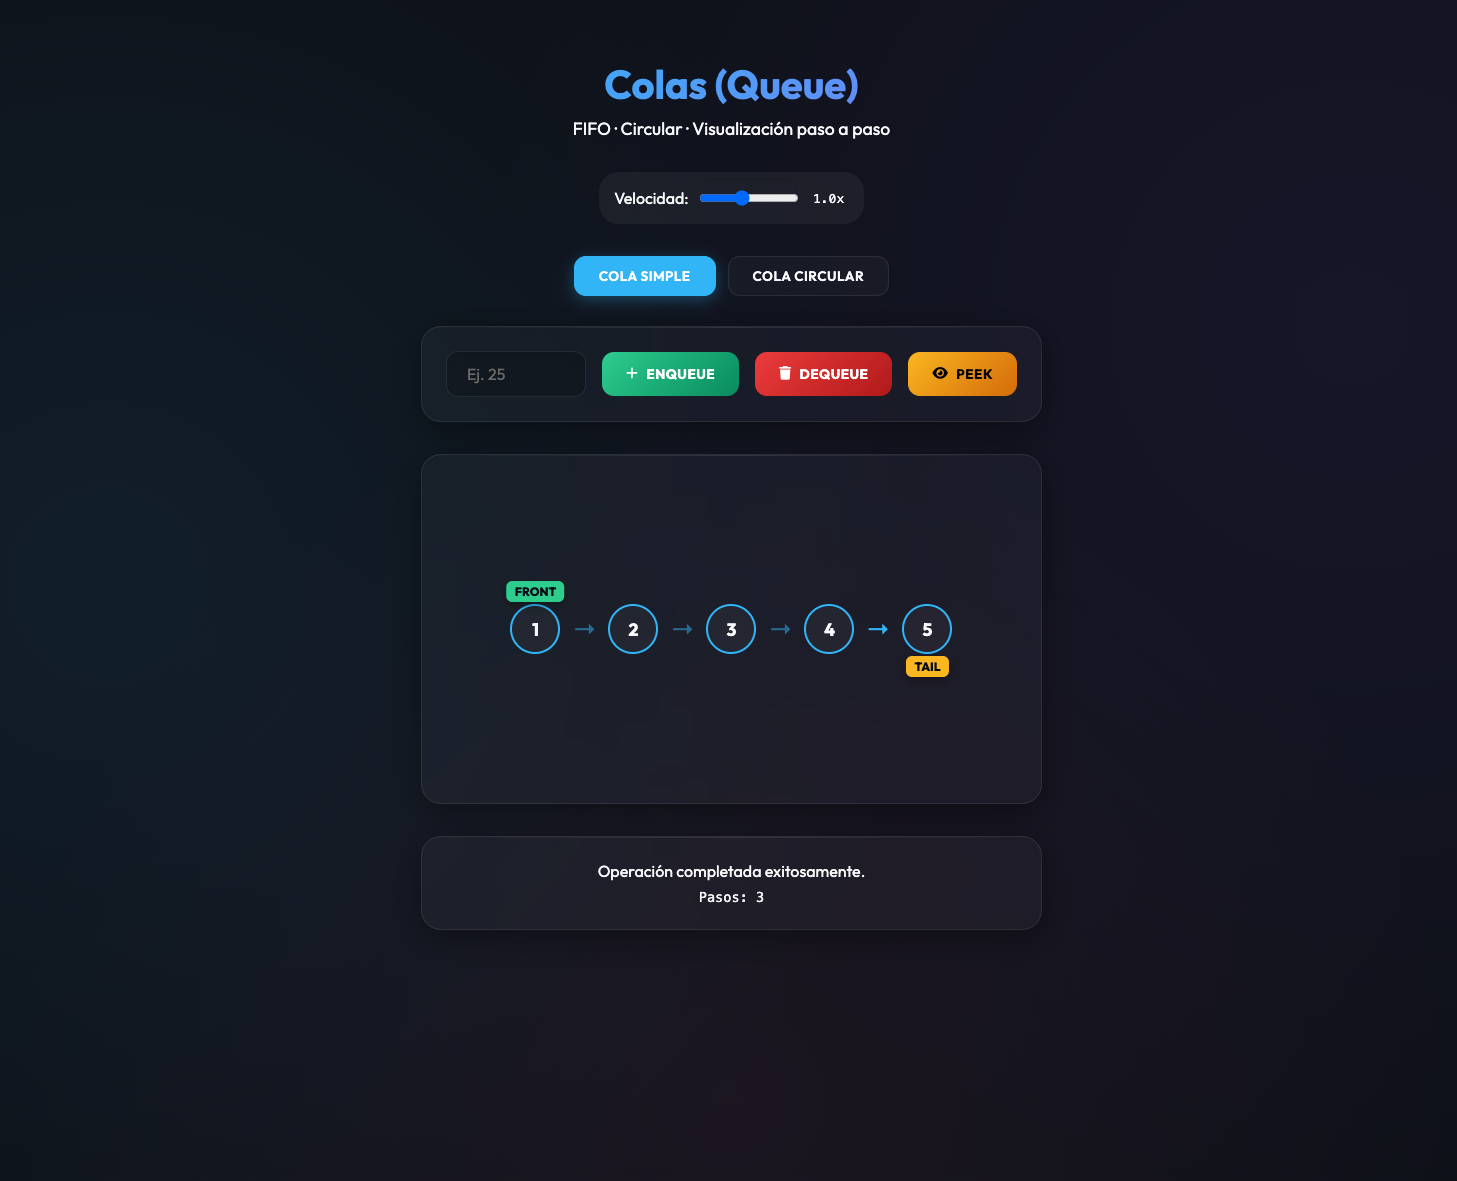
\includegraphics[width=0.85\textwidth]{imagenes/simulador_cola_simple.png}
  \caption{Cola Simple FIFO}
  \label{fig:cola_simple}
\end{figure}

\begin{figure}[!ht]
  \centering
  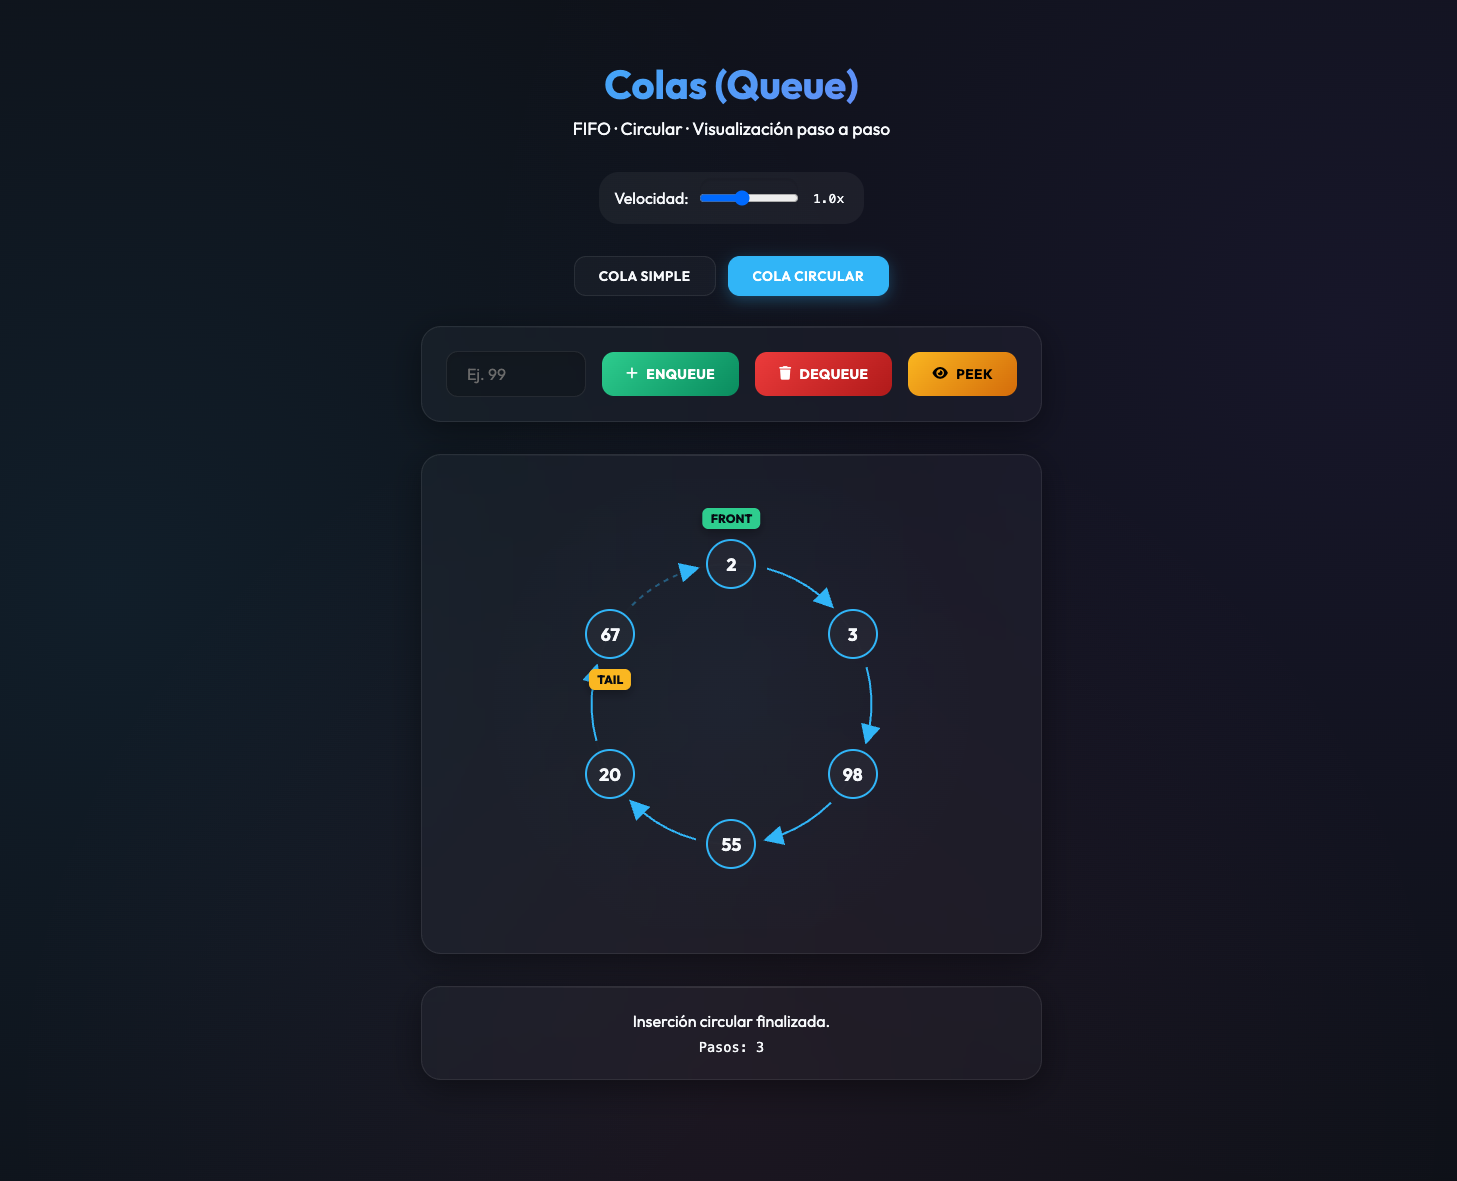
\includegraphics[width=0.85\textwidth]{imagenes/simulador_cola_circular.png}
  \caption{Cola Circular}
  \label{fig:cola_circular}
\end{figure}

\begin{figure}[!ht]
  \centering
  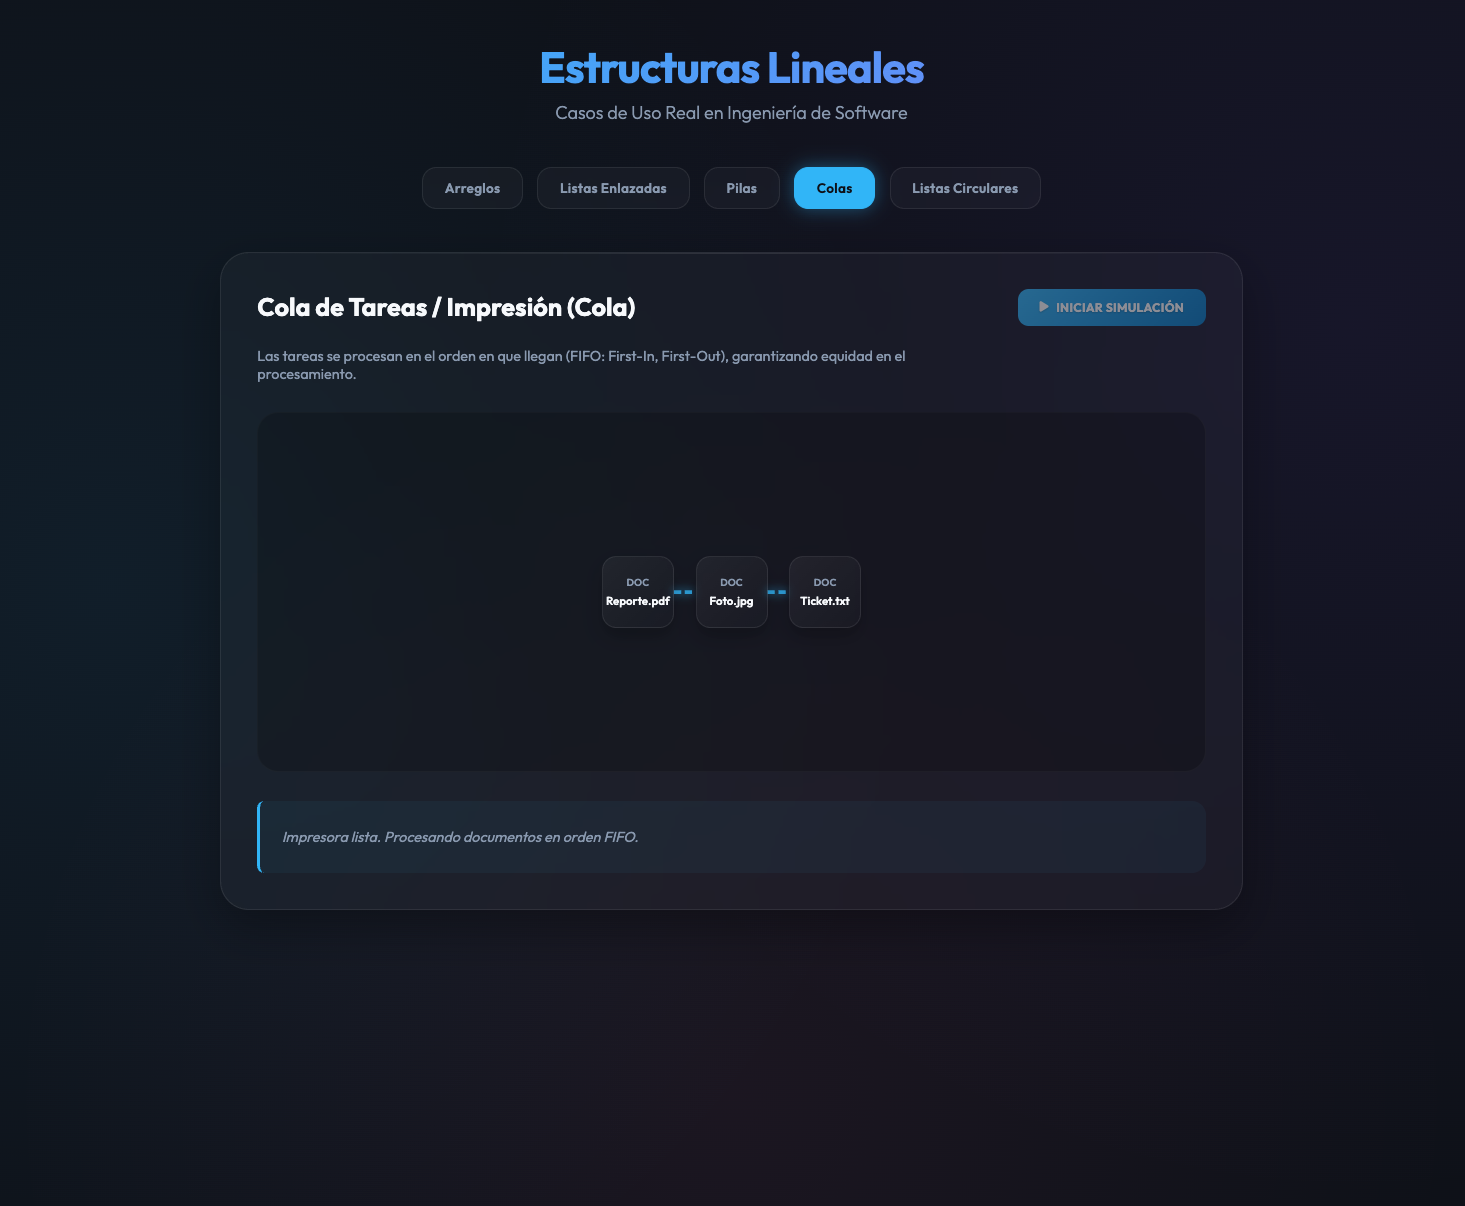
\includegraphics[width=0.85\textwidth]{imagenes/simulador_casos_uso_colas.png}
  \caption{Casos de Uso en Colas}
  \label{fig:casos_uso_colas}
\end{figure}

\clearpage

\subsubsection*{D) Simuladores de Estructuras Jerárquicas y No Lineales (Árboles, Montículos y Tablas Hash)}

\noindent \textbf{Árboles Binarios en \texttt{/proyectos/07\_arboles}:} Visualizador dinámico que autogestiona el espacio y distribución física de las hojas y ramas en pantalla, permitiendo interactuar con inserciones, eliminaciones, balanceos AVL y recorridos recursivos.

\begin{figure}[!ht]
  \centering
  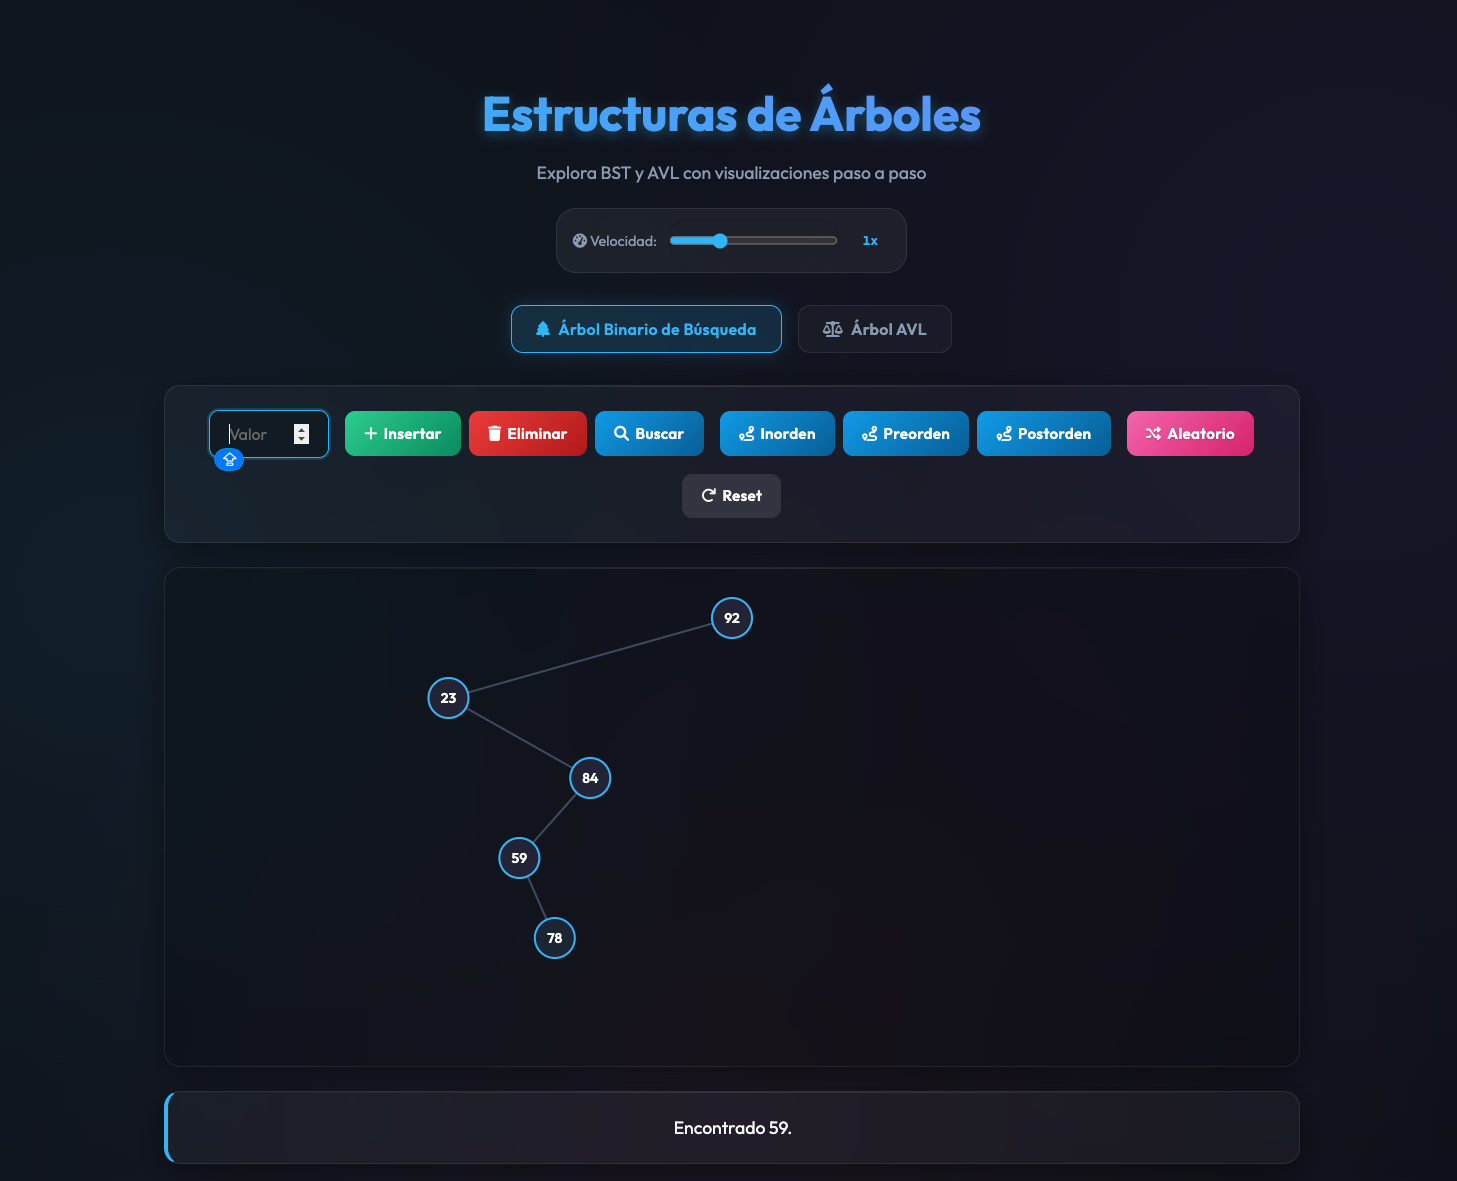
\includegraphics[width=0.85\textwidth]{imagenes/simulador_abb.png}
  \caption{Simulador de Árbol Binario de Búsqueda BST}
  \label{fig:sim_abb}
\end{figure}
\newpage
\begin{figure}[!ht]
  \centering
  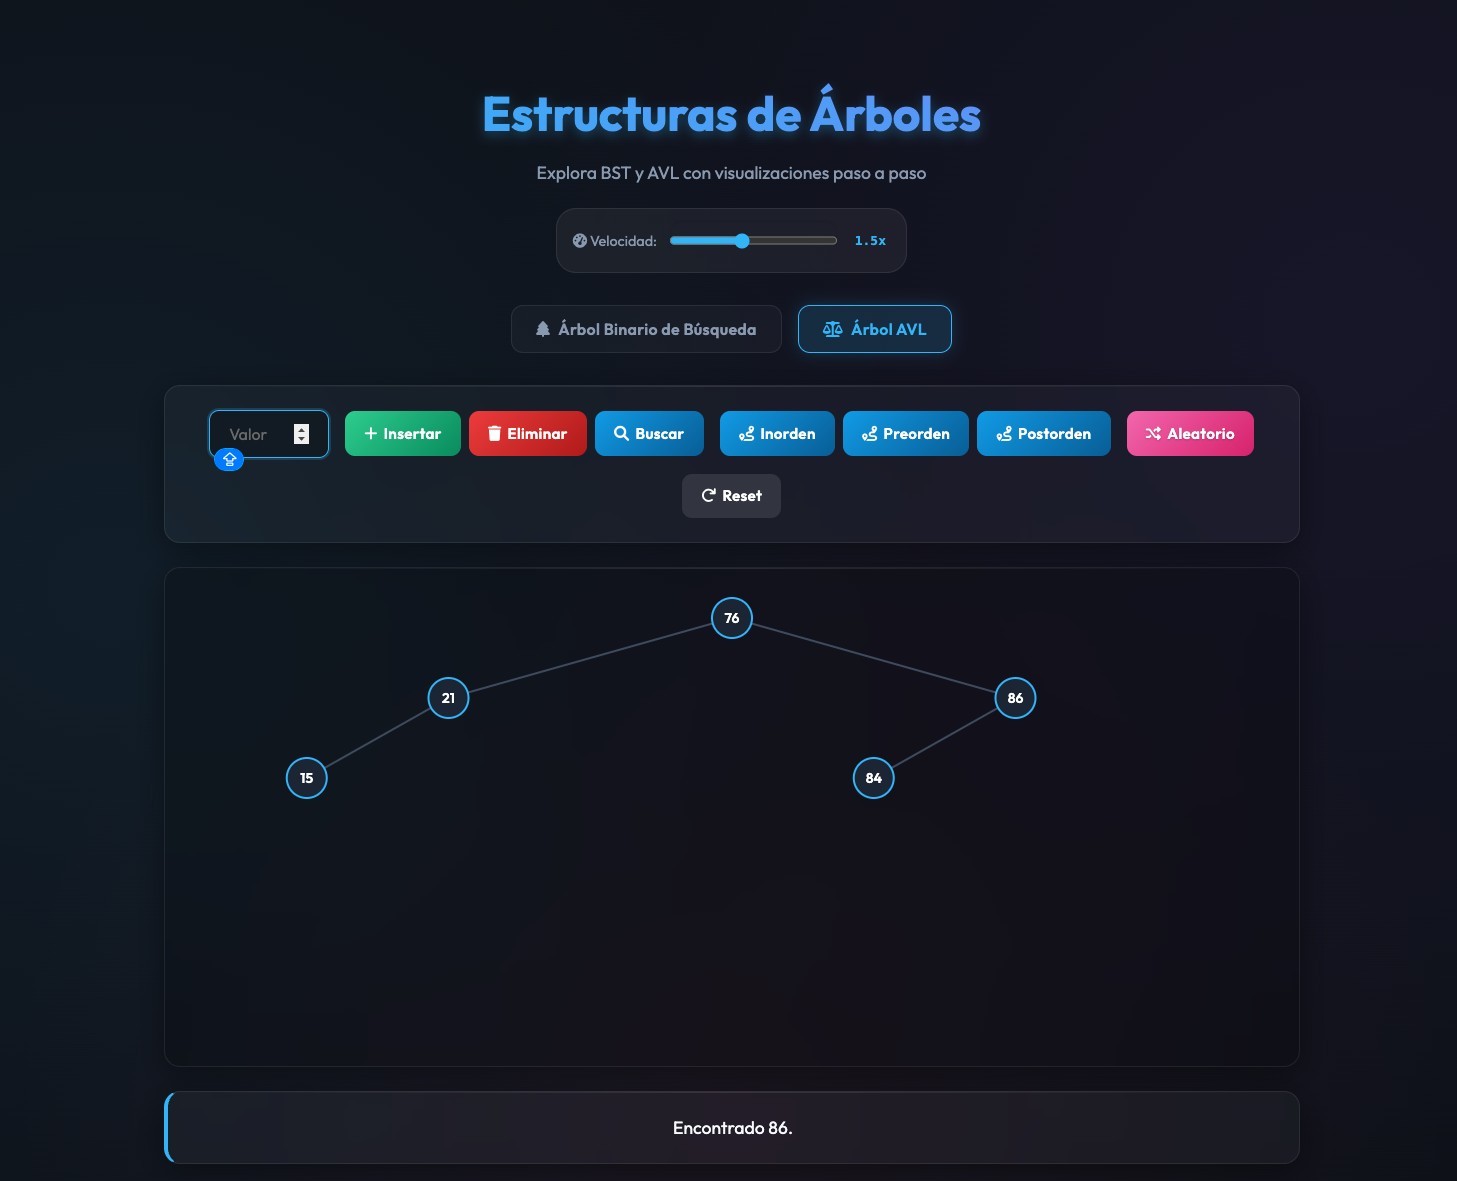
\includegraphics[width=0.85\textwidth]{imagenes/simulador_avl.png}
  \caption{Simulador de Árbol AVL Balanceado}
  \label{fig:sim_avl}
\end{figure}
\newpage

\noindent \textbf{Montículos y Tablas Hash en \texttt{/proyectos/08\_heaps} y \texttt{/proyectos/09\_hash}:} Representaciones del orden de prioridad de un montículo y visualización física de la resolución de colisiones mediante encadenamiento o direccionamiento abierto.

\begin{figure}[!ht]
  \centering
  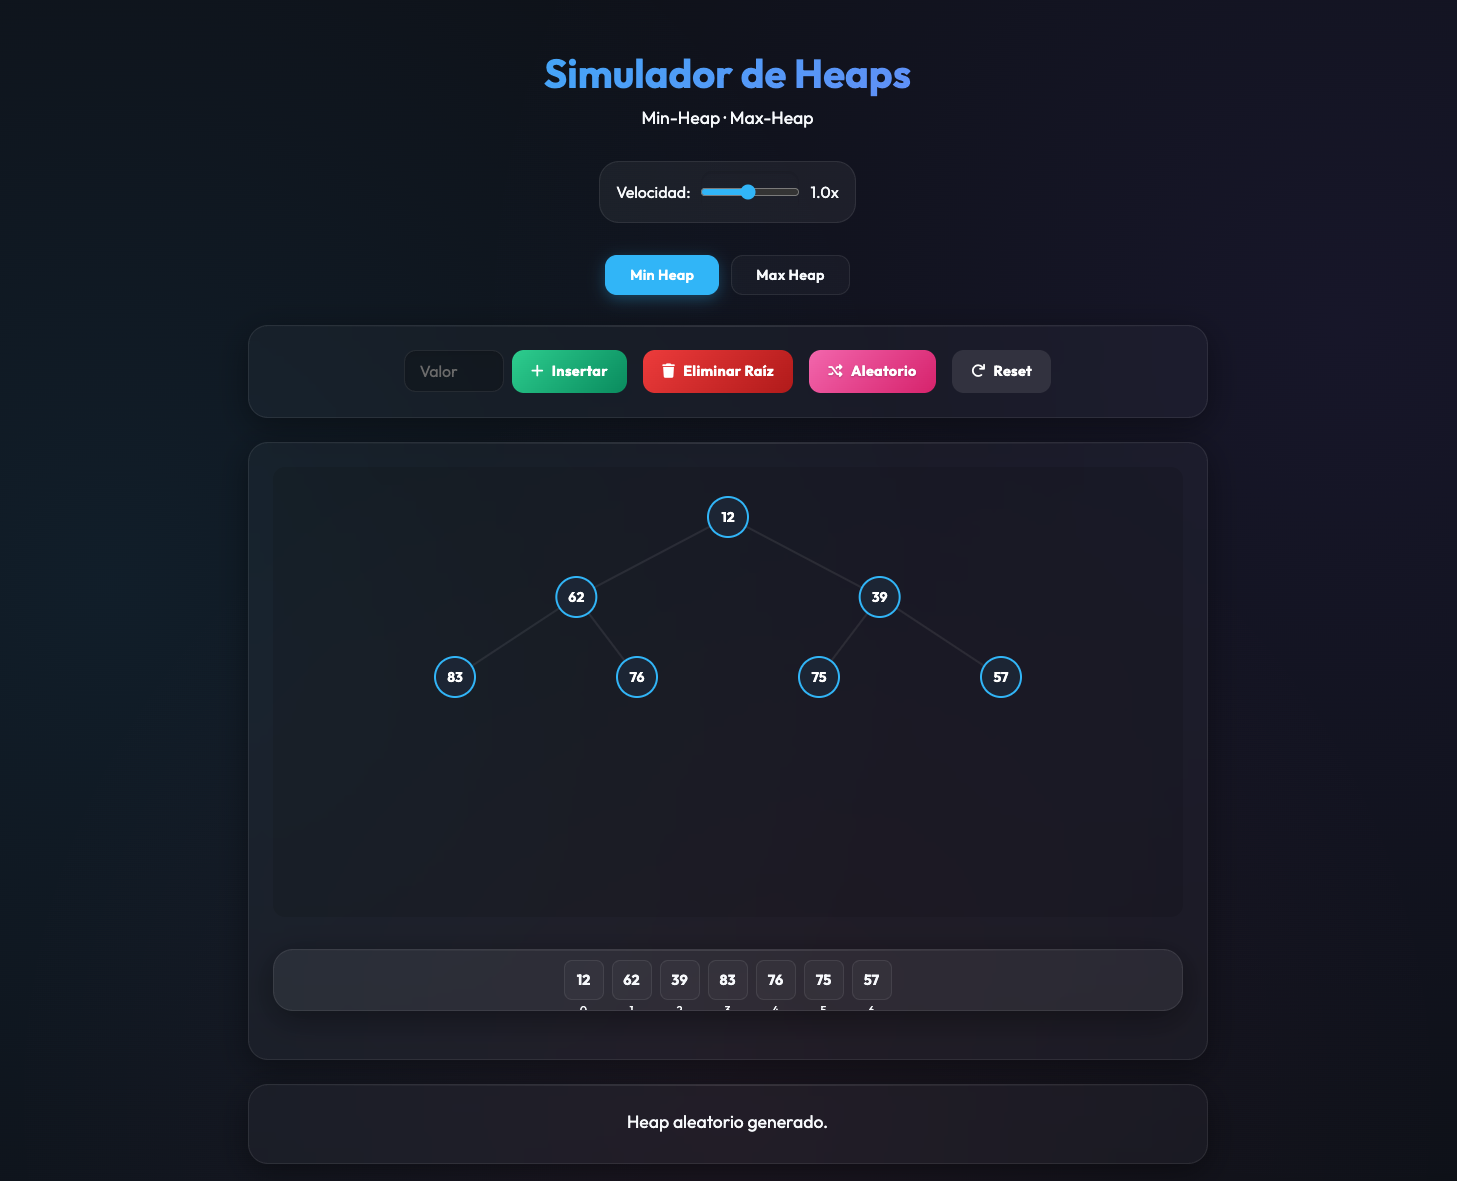
\includegraphics[width=0.85\textwidth]{imagenes/simulador_heaps.png}
  \caption{Montículos de Prioridad}
  \label{fig:sim_heaps}
\end{figure}

\begin{figure}[!ht]
  \centering
  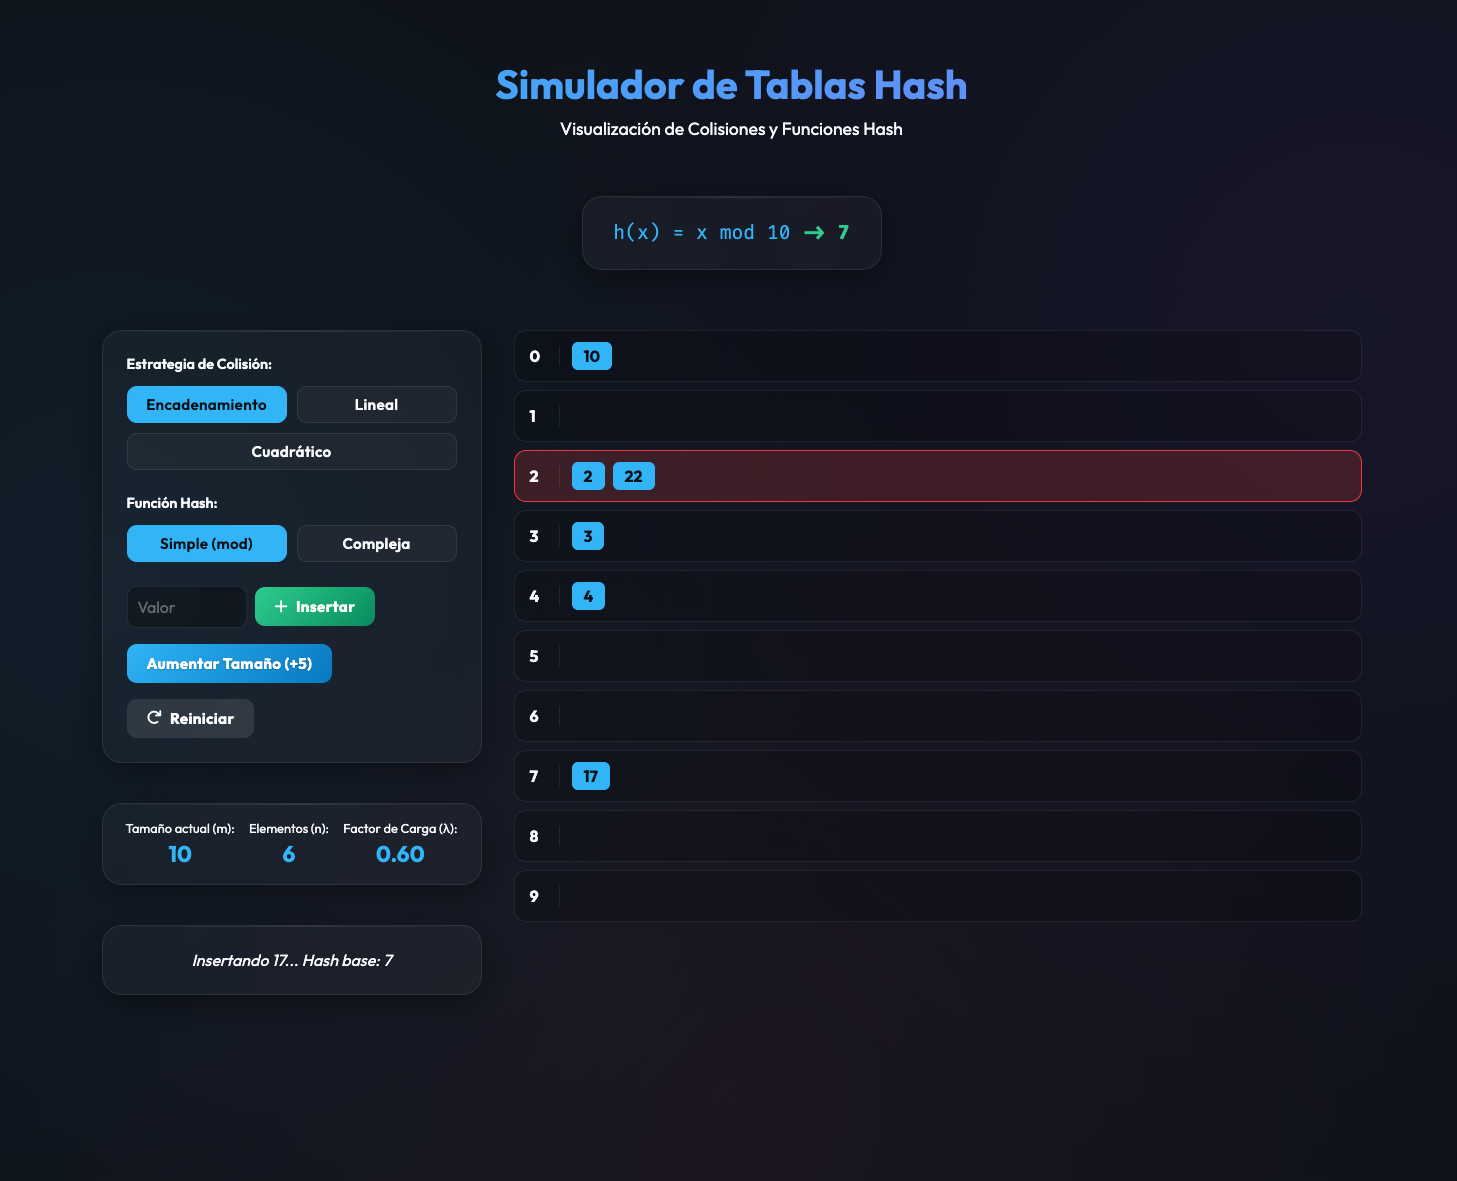
\includegraphics[width=0.85\textwidth]{imagenes/simulador_hash.png}
  \caption{Manejo de Colisiones en Tabla Hash}
  \label{fig:sim_hash}
\end{figure}

\clearpage

\subsubsection*{E) Visualizadores de Gráficas y Algoritmos de Caminos Mínimos}

\noindent \textbf{Gráficas en \texttt{/proyectos/10\_graficas}:} Representación interactiva de vértices, conexiones dirigidas y ponderadas, y la ejecución paso a paso del recorrido de Dijkstra para encontrar el camino más corto.

\begin{figure}[!ht]
  \centering
  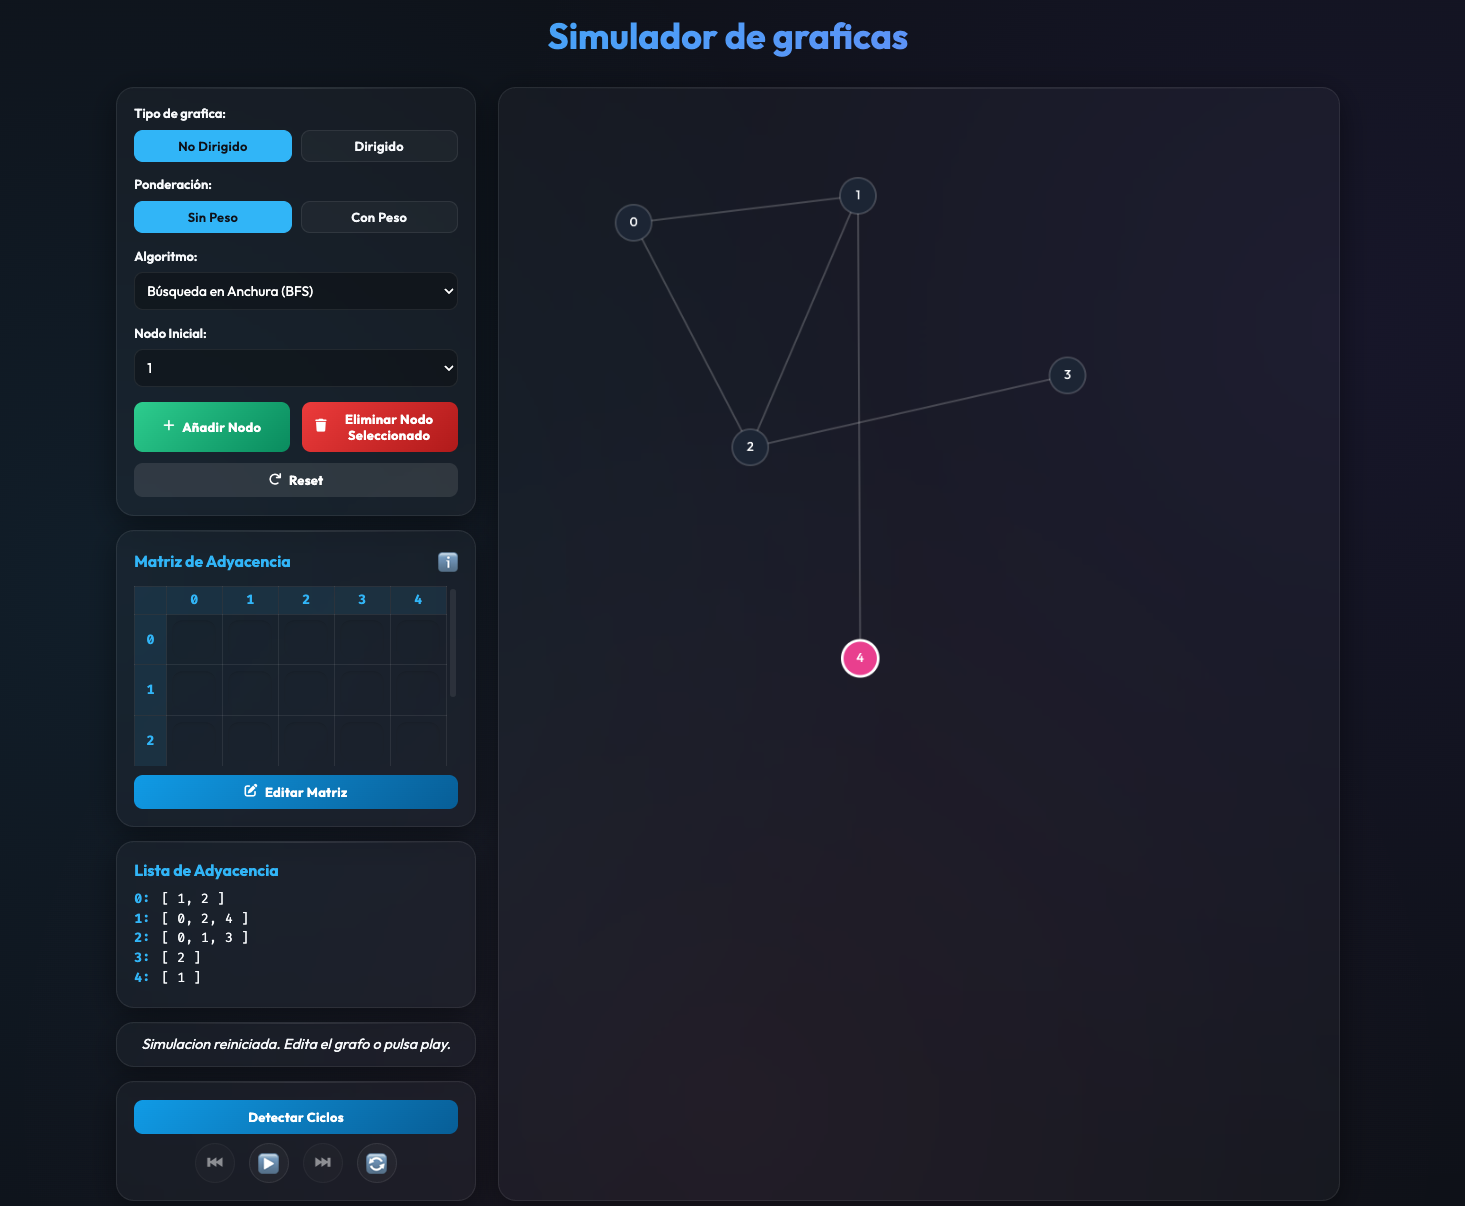
\includegraphics[width=0.85\textwidth]{imagenes/simulador_graficas.png}
  \caption{Visualizador de Gráficas y Vértices}
  \label{fig:sim_graficas}
\end{figure}

\begin{figure}[!ht]
  \centering
  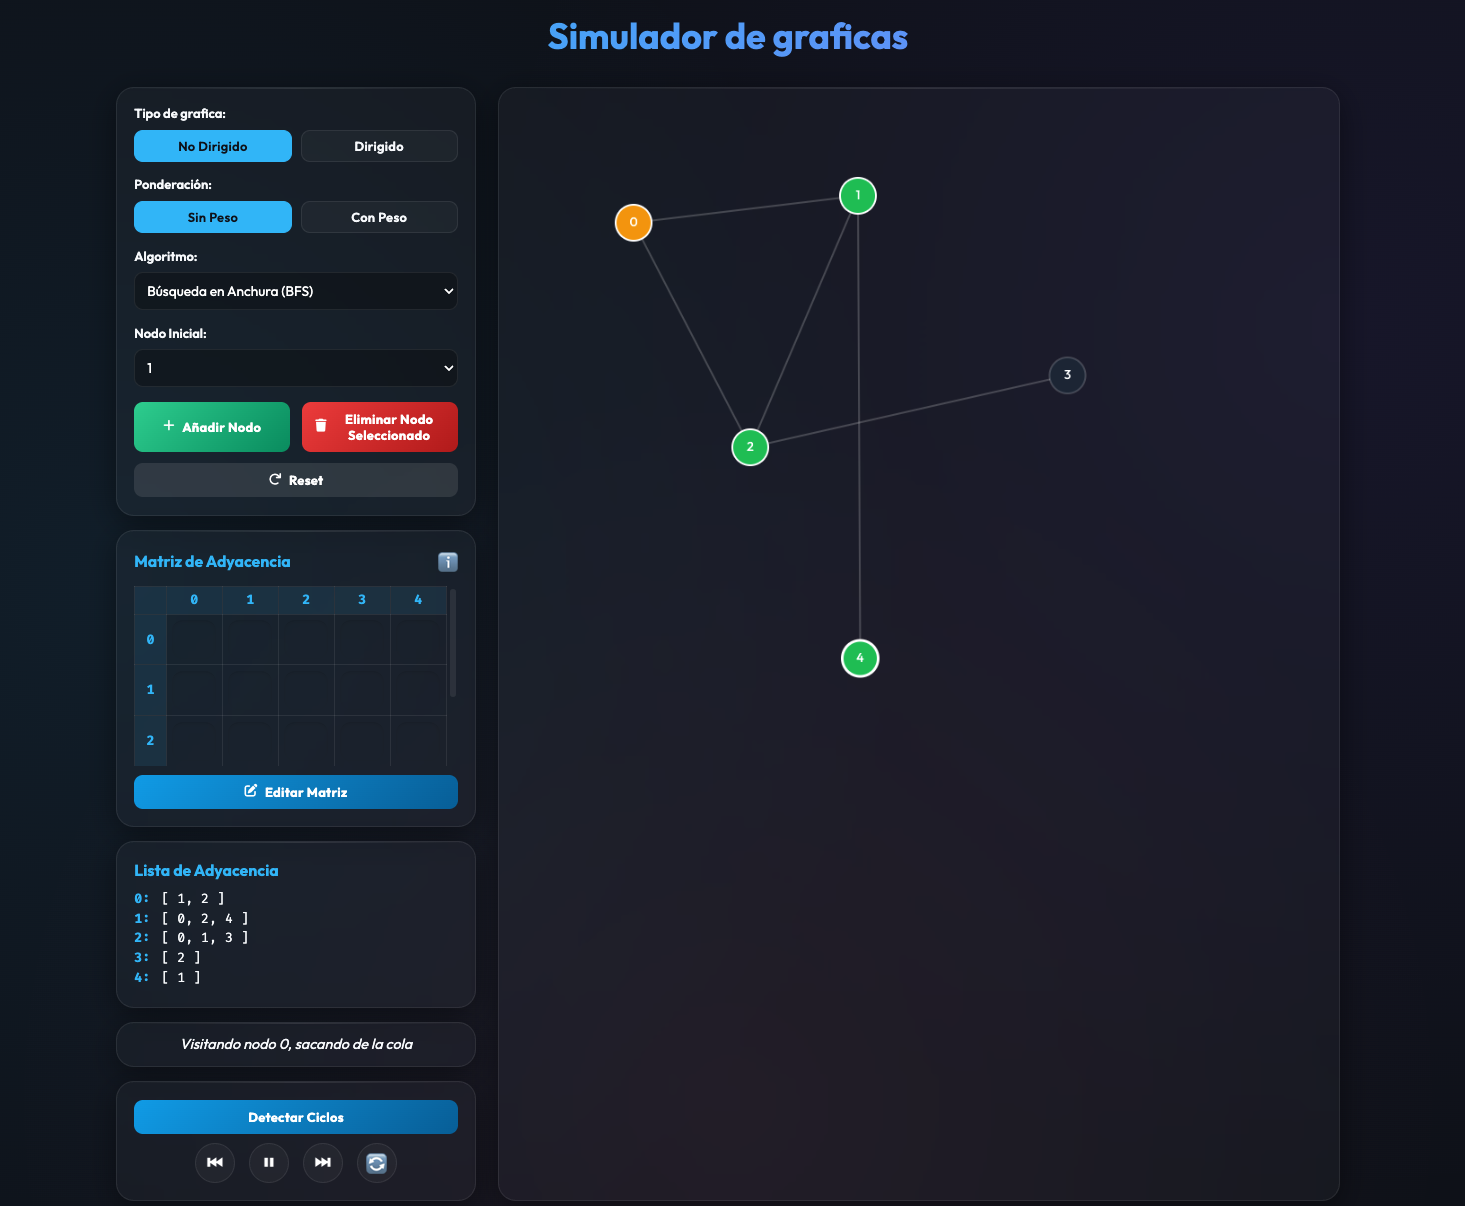
\includegraphics[width=0.85\textwidth]{imagenes/simulador_graficas_recorrido.png}
  \caption{Simulación de Recorridos}
  \label{fig:sim_graficas_recorrido}
\end{figure}




\begin{figure}[!ht]
  \centering
  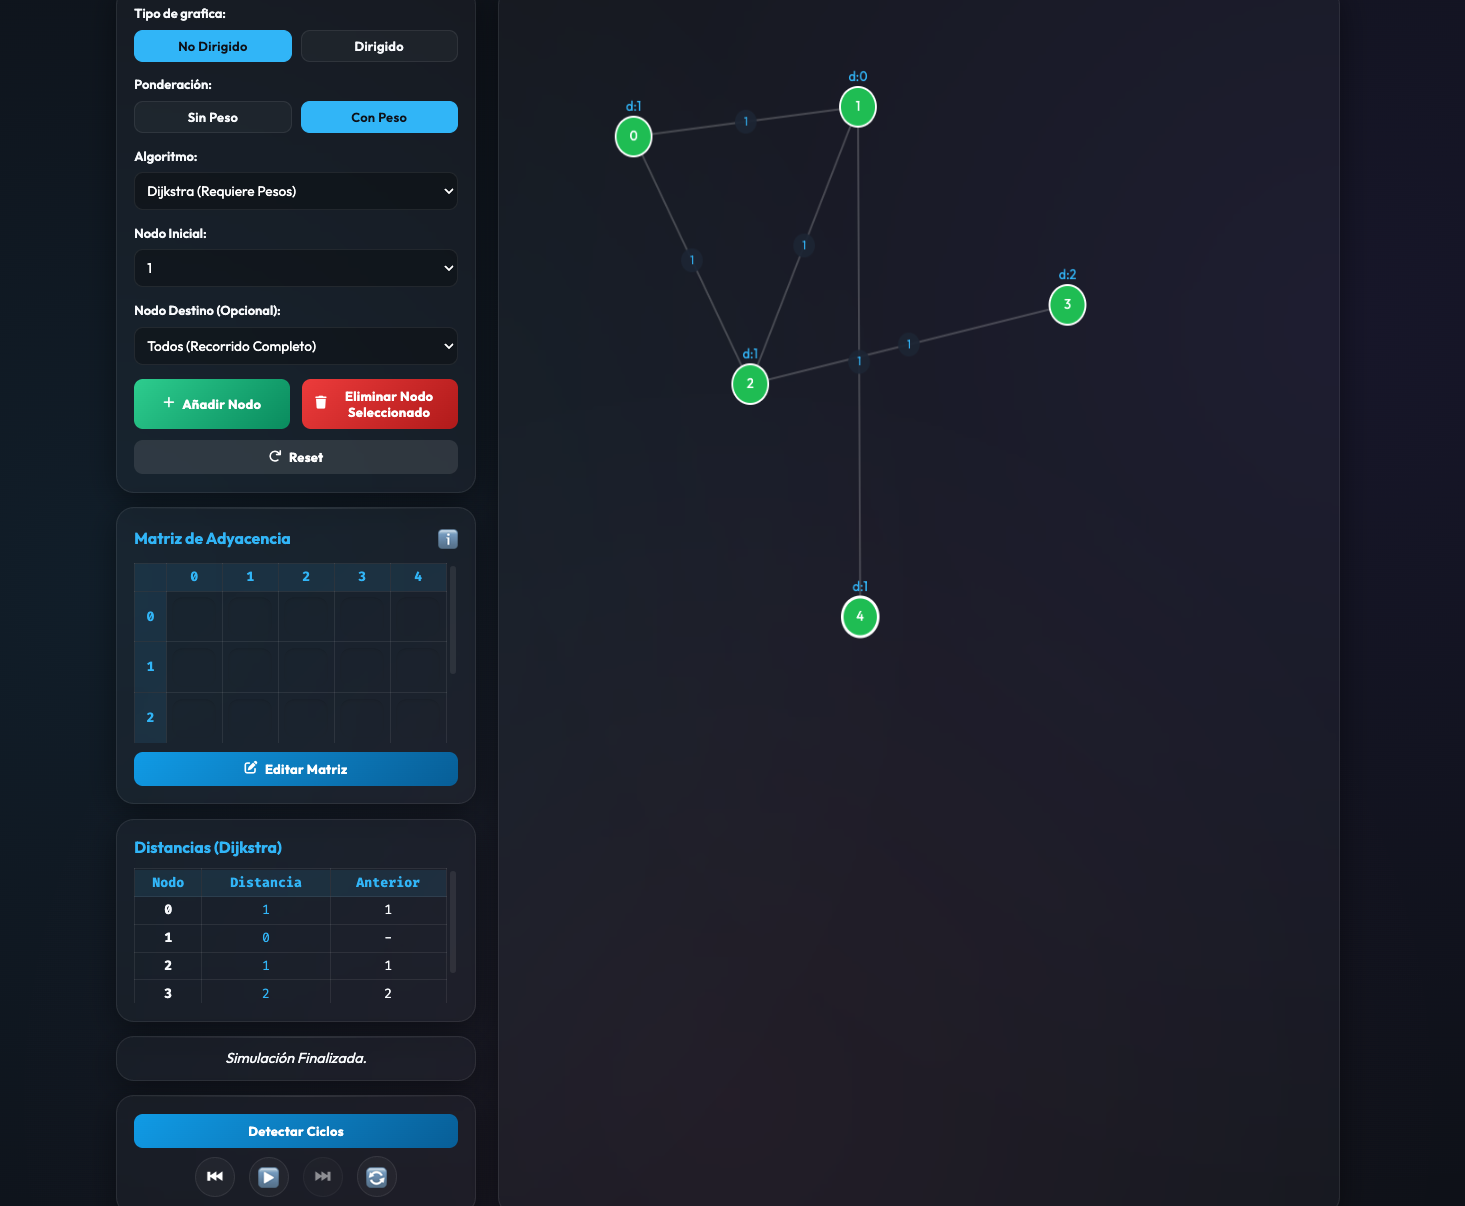
\includegraphics[width=0.85\textwidth]{imagenes/simulador_graficas_dijkstra.png}
  \caption{Dijkstra para Caminos Mínimos}
  \label{fig:sim_graficas_dijkstra}
\end{figure}

\clearpage

\subsubsection*{F) Algoritmos de Búsqueda, Ordenamiento y Backtracking}

\noindent \textbf{Algoritmos de Ordenamiento y Búsqueda:} Representación visual interactiva mediante barras dinámicas de alturas que comparan el coste y la velocidad de los diferentes ordenamientos clásicos e ilustran las búsquedas lineales y binarias.

\begin{figure}[!ht]
  \centering
  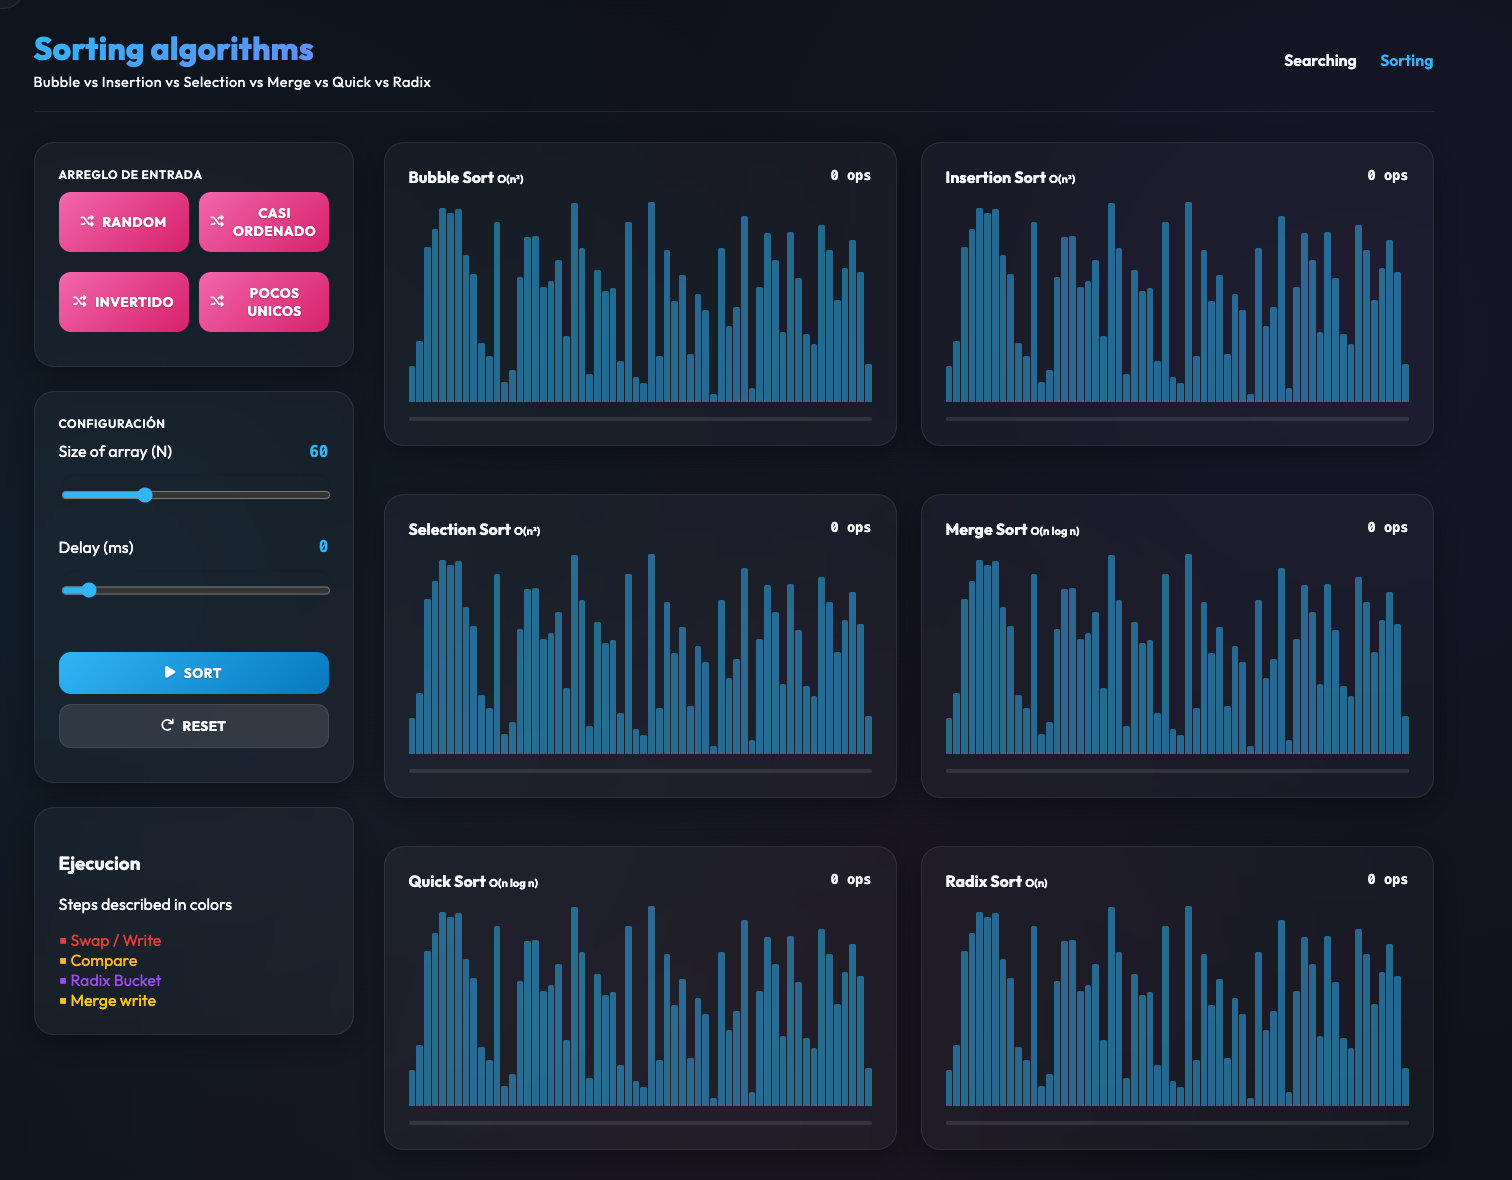
\includegraphics[width=0.85\textwidth]{imagenes/simulador_sorting_before.png}
  \caption{Ordenación en Estado Inicial}
  \label{fig:sorting_before}
\end{figure}
\newpage
\begin{figure}[!ht]
  \centering
  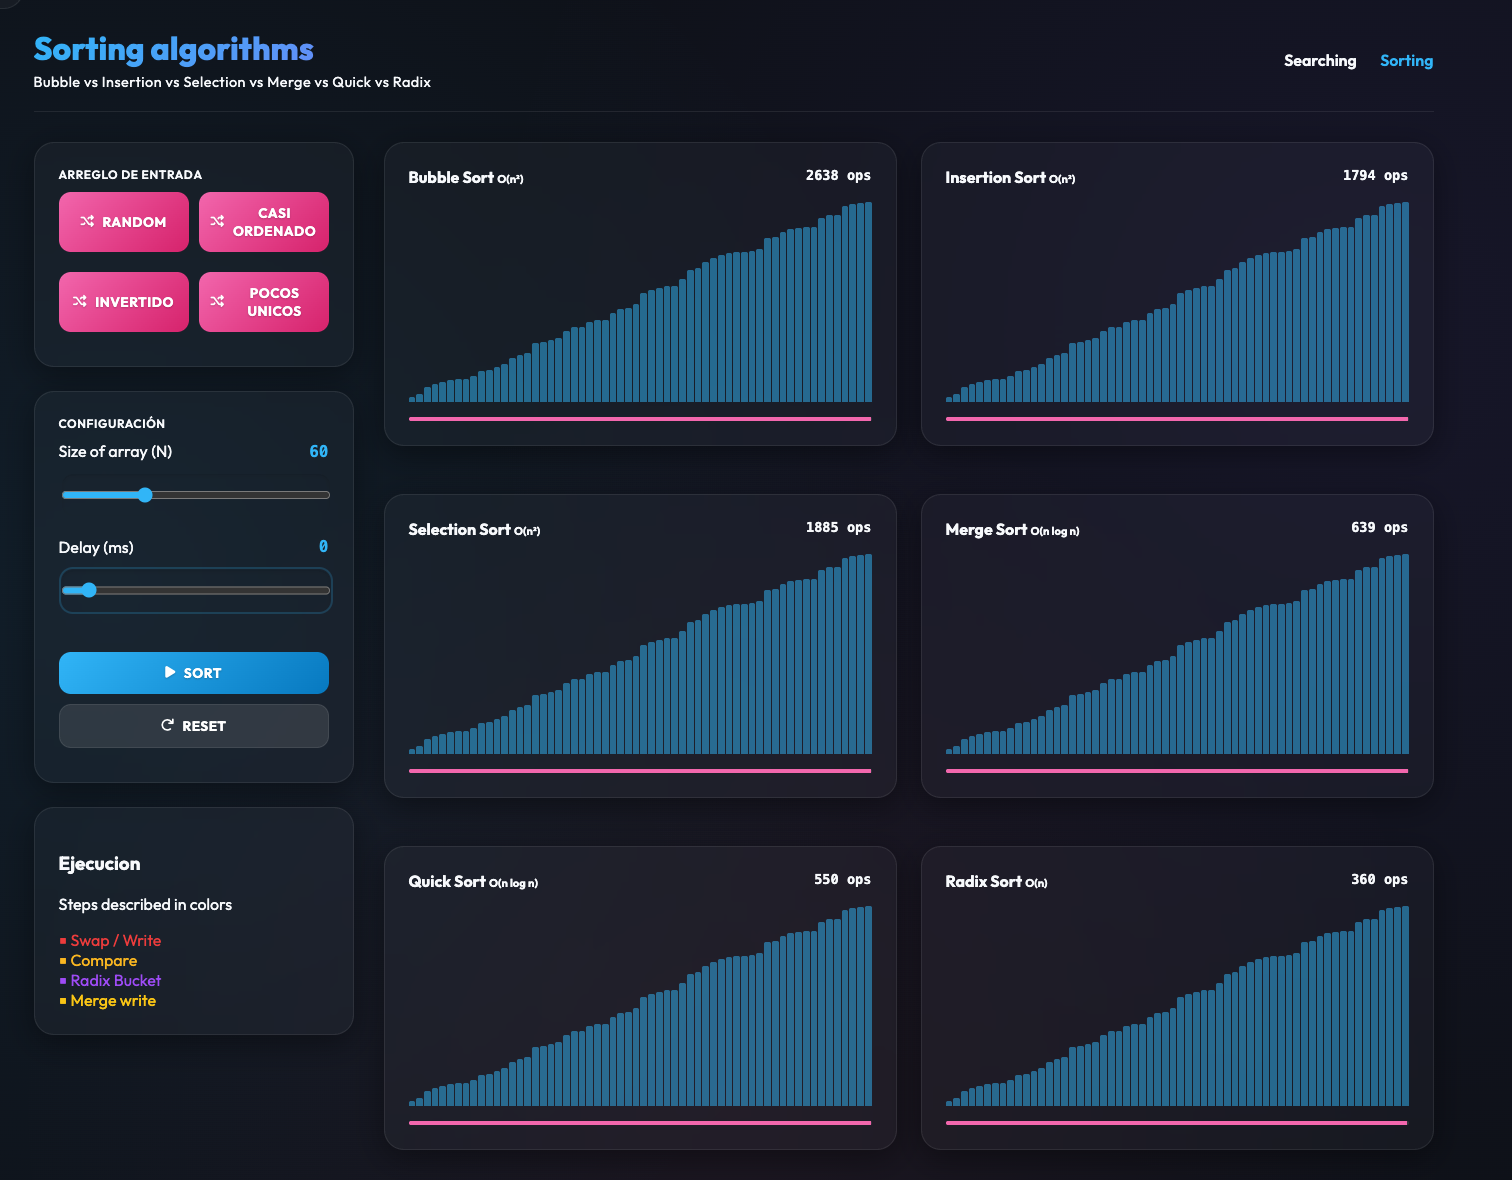
\includegraphics[width=0.85\textwidth]{imagenes/simulador_sorting_after.png}
  \caption{Ordenación Completada}
  \label{fig:sorting_after}
\end{figure}
\newpage

\begin{figure}[!ht]
  \centering
  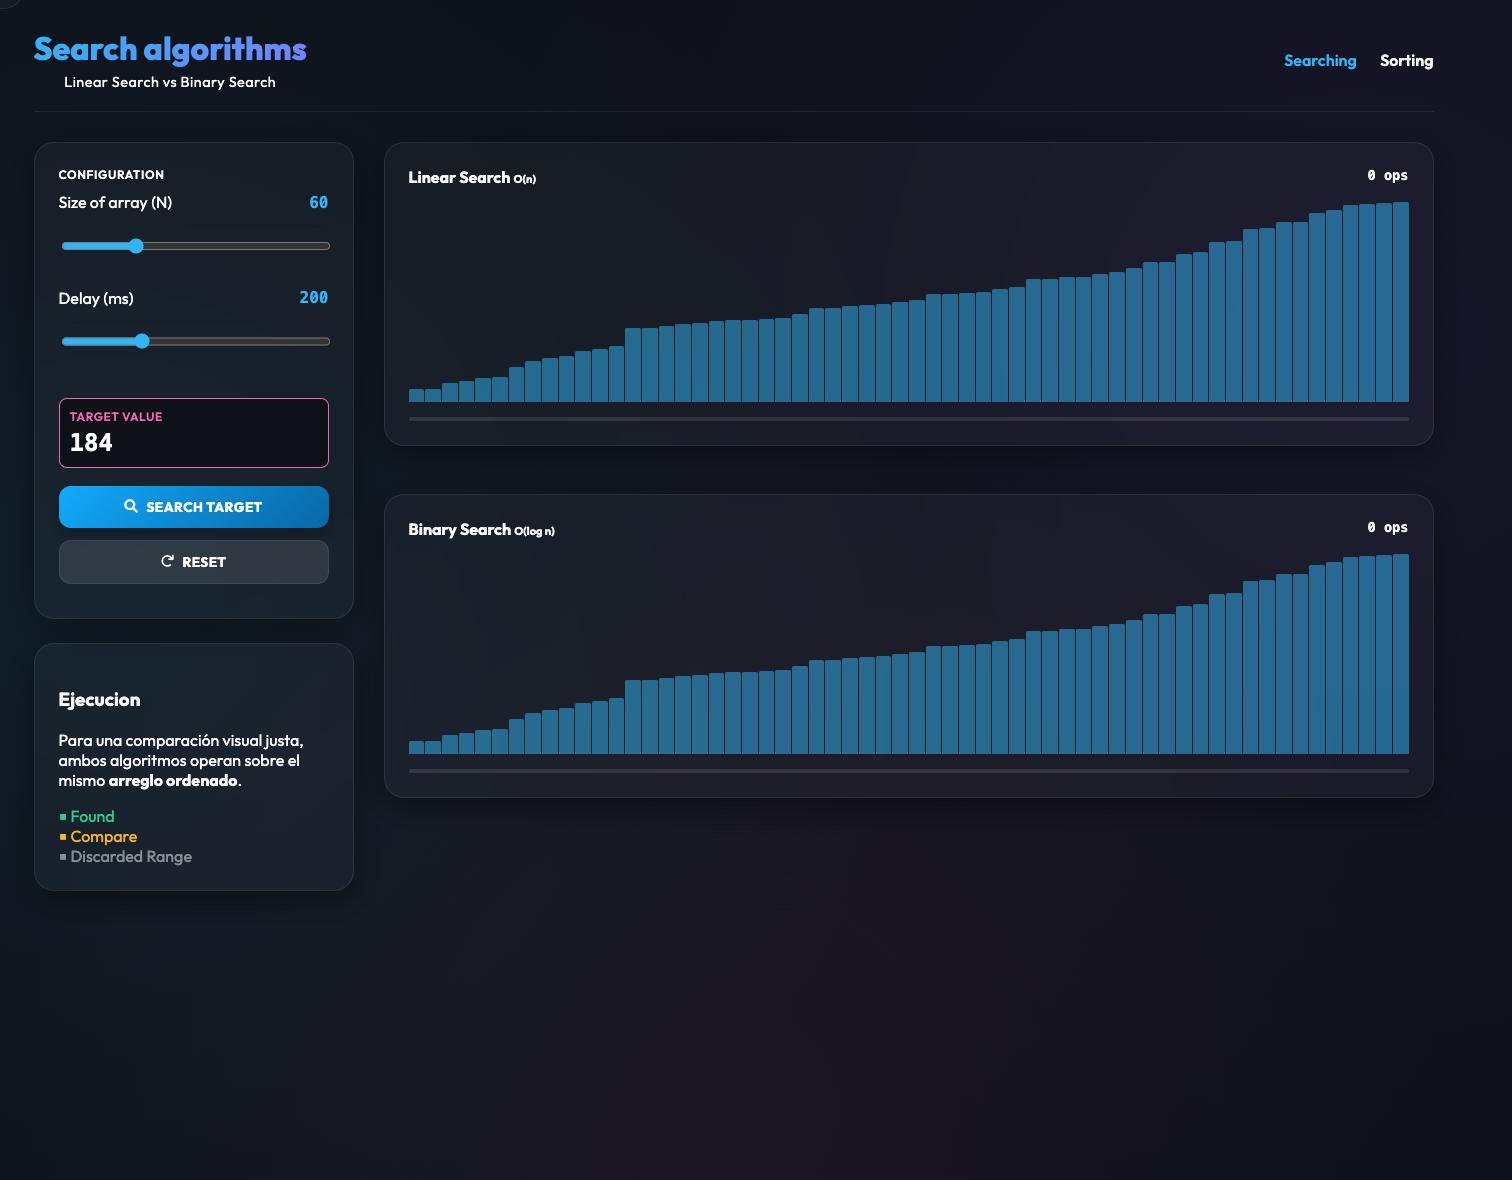
\includegraphics[width=0.85\textwidth]{imagenes/simulador_searching_before.png}
  \caption{Búsqueda en Estado Inicial}
  \label{fig:searching_before}
\end{figure}
\newpage
\begin{figure}[!ht]
  \centering
  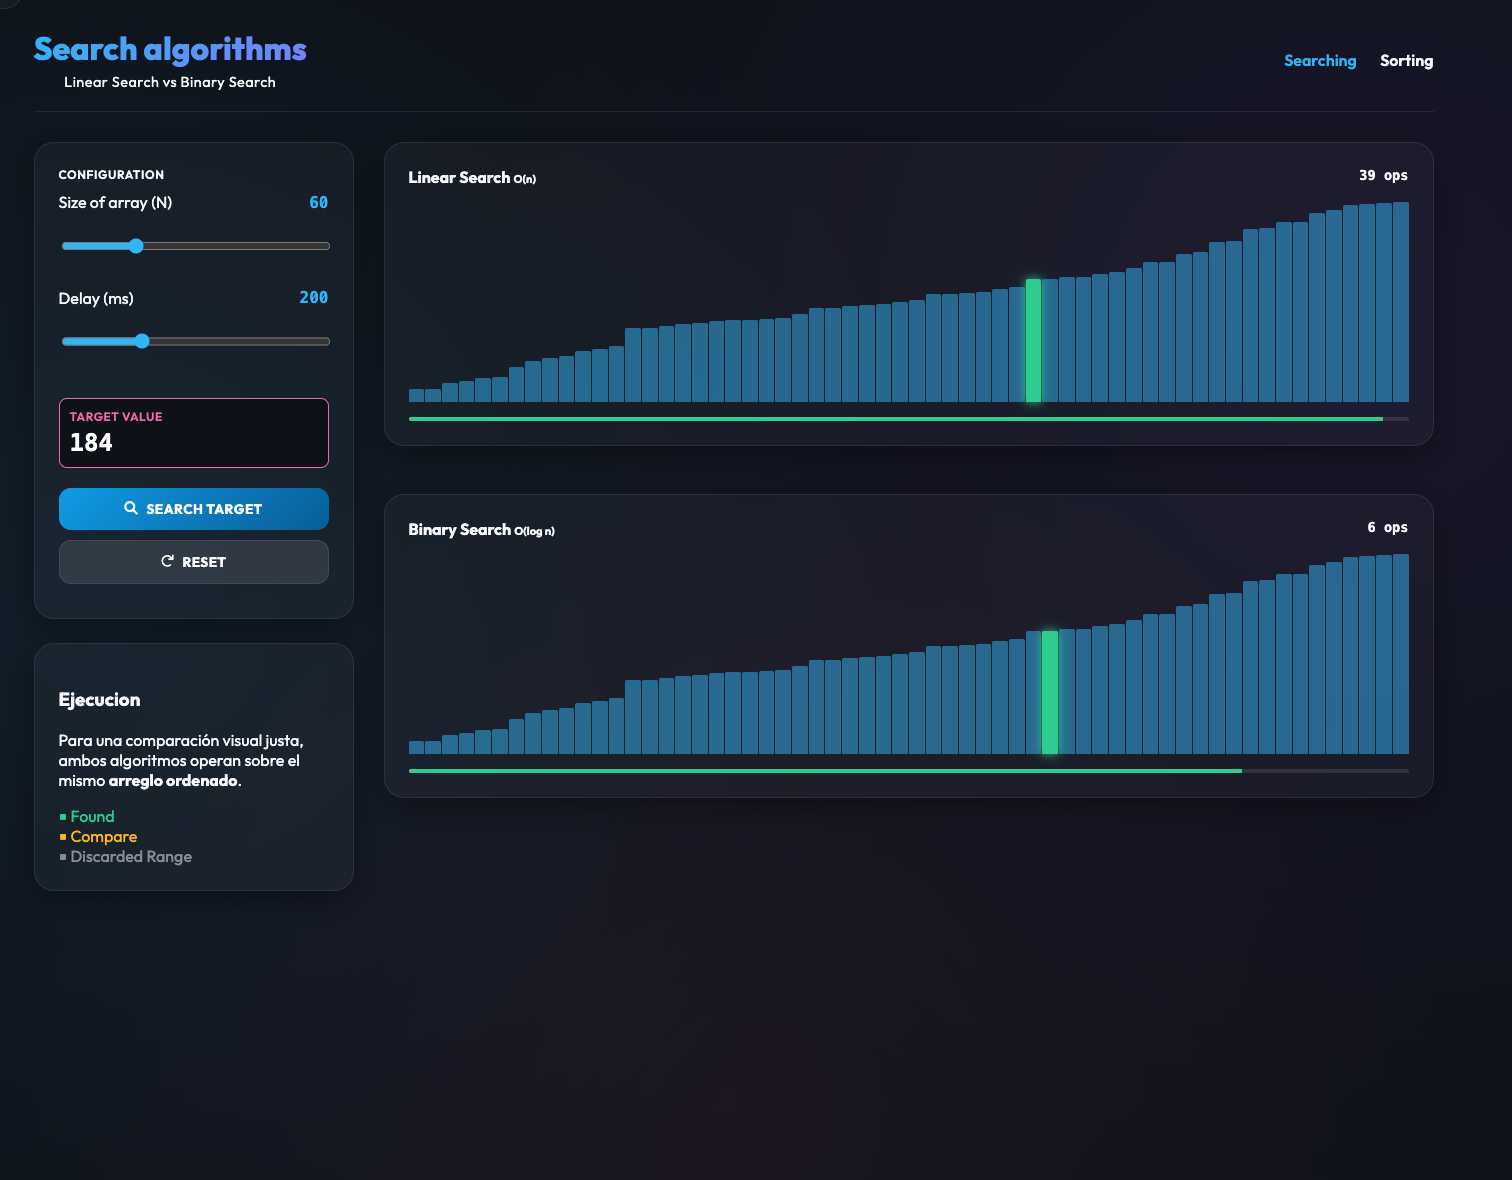
\includegraphics[width=0.85\textwidth]{imagenes/simulador_searching_after.png}
  \caption{Elemento Encontrado}
  \label{fig:searching_after}
\end{figure}
\newpage
\noindent \textbf{Algoritmo de Backtracking:} Muestra de manera sumamente clara la generación de la pila de llamadas recursivas y el cómo el algoritmo de backtracking va explorando todas las posibilidades hasta encontrar una solución. En este caso en un laberinto.

\begin{figure}[!ht]
  \centering
  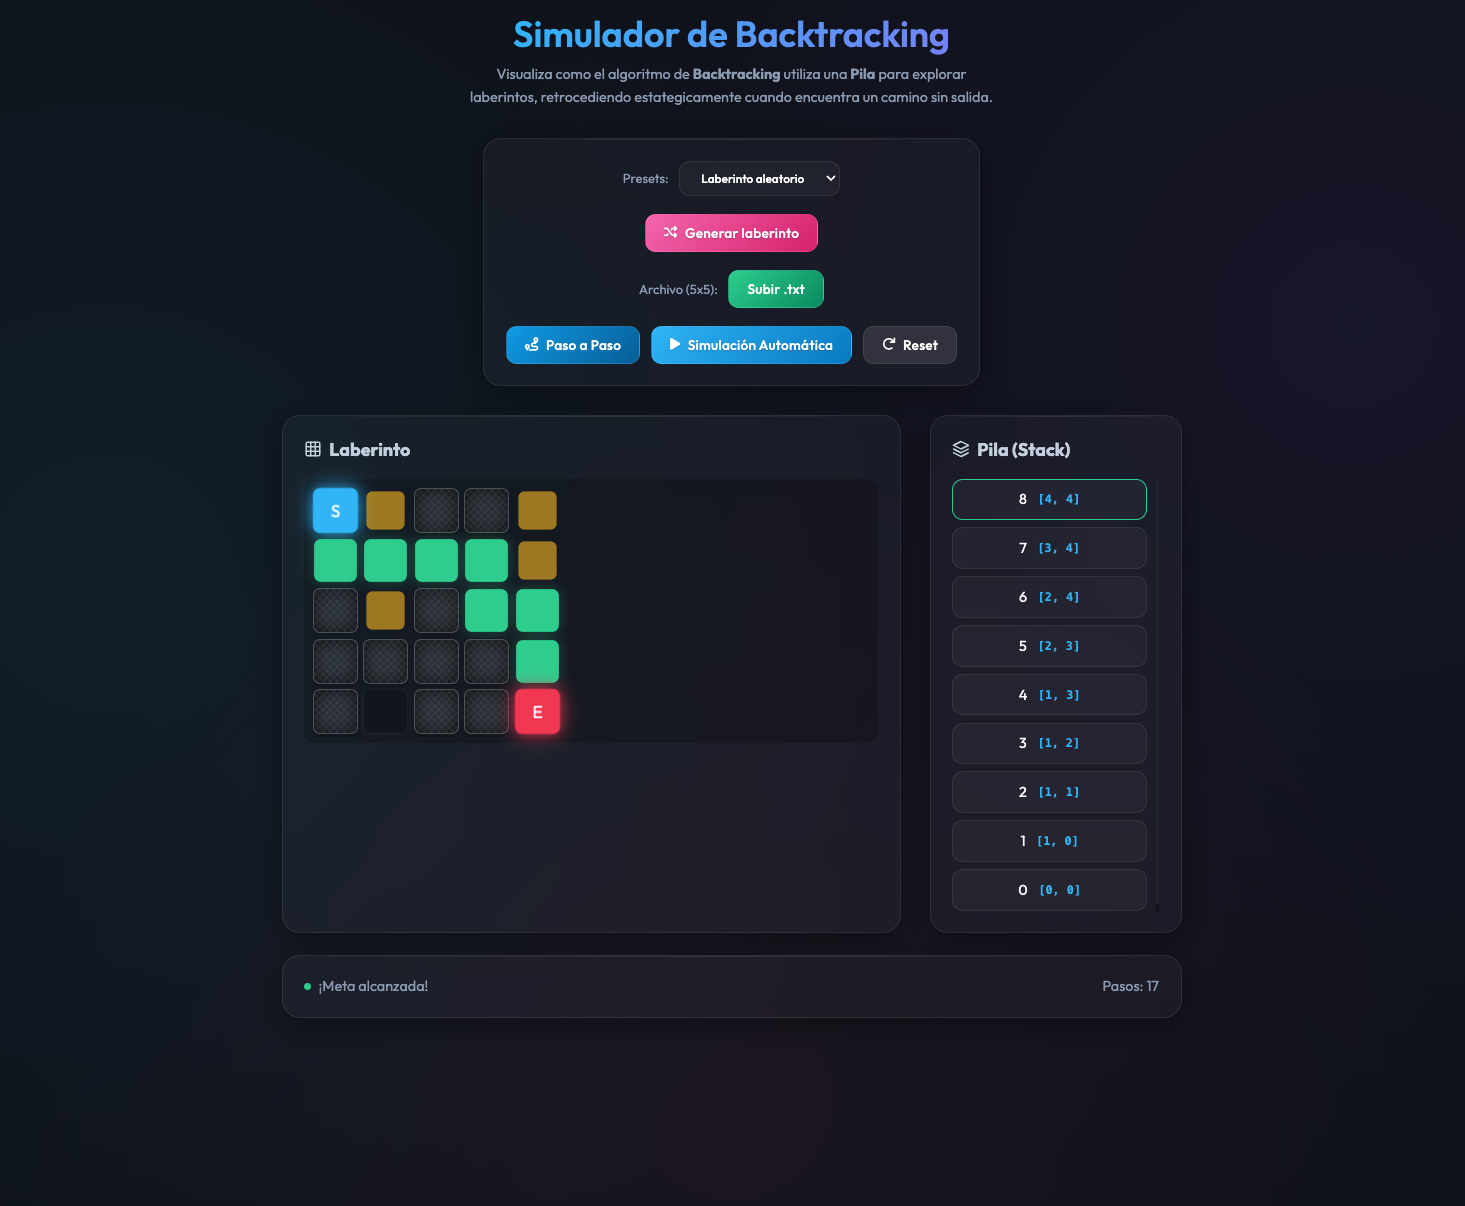
\includegraphics[width=0.85\textwidth]{imagenes/simulador_backtracking.png}
  \caption{Simulador de Backtracking e Interfaz del Problema de N-Reinas}
  \label{fig:sim_backtracking}
\end{figure}

\clearpage

\section*{8. Pruebas de Calidad, Validación e Integración}
\addcontentsline{toc}{section}{8. Pruebas de Calidad, Validación e Integración}

Para certificar la robustez de los ejercicios prácticos se implementó un flujo continuo de validación local mediante comandos nativos de Bazel:

\begin{verbatim}
# Comando ejecutado para validar todas las pruebas unitarias
# y garantizar 0 errores de compilación
bazel test //...
\end{verbatim}

La suite de pruebas ejecuta decenas de aserciones lógicas que validan:
\begin{itemize}
    \item La correcta gestión de punteros de las listas bajo condiciones extremas.
    \item El manejo estricto de excepciones lógicas (como desbordamiento o subdesbordamiento).
    \item La correctitud de los algoritmos de ordenación.
\end{itemize}

\begin{figure}[!ht]
  \centering
  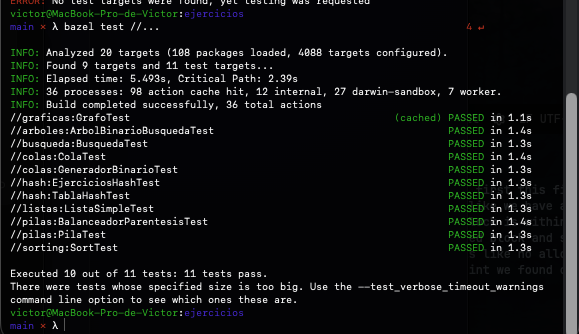
\includegraphics[width=0.85\textwidth]{imagenes/bazel_command.png}
  \caption{Ejecución Exitosa de la Suite de Pruebas con Bazel}
  \label{fig:bazel_command}
\end{figure}

\section*{9. Retos Técnicos, Experiencia Formativa y Autoaprendizaje}
\addcontentsline{toc}{section}{9. Retos Técnicos, Experiencia Formativa y Autoaprendizaje}

El desarrollo de este Servicio Social representó una oportunidad invaluable de autoaprendizaje que sin duda complementó la educación que adquirí a lo largo de mi licenciatura. Entre los principales aprendizajes y retos superados destacan:

\begin{enumerate}
    \item \textbf{Gestión Asíncrona en el Frontend:} Diseñar animaciones que se ejecutaran en paralelo con la lógica del algoritmo de estructuras de datos requirió un dominio avanzado del bucle de eventos (\emph{event loop}) de JavaScript y del uso sistemático de \texttt{Promises} y funciones \texttt{async/await} para poder pausar la ejecución en puntos clave sin congelar la interfaz de usuario.
    \item \textbf{Dominio de Sistemas de Construcción Modernos:} Estructurar proyectos Java utilizando Bazel obligó a comprender las bases de la compilación reproducible y hermética, conocimientos altamente cotizados en la industria del desarrollo de software de gran escala.
    \item \textbf{Didáctica y Síntesis Pedagógica:} Traducir conceptos matemáticos abstractos a simulaciones visuales intuitivas y guías sencillas fortaleció de gran manera mis habilidades de comunicación y síntesis, permitiéndome aprender a diseñar software pensando siempre en la experiencia del usuario final (en este caso, estudiantes de semestres introductorios).
    \item \textbf{Diseño de interfaces:} Durante mi licenciatura siempre evité trabajar con la interfaz de usuario, sin embargo este proyecto me permitió entender la importancia de un buen diseño de interfaz y cómo irla mejorando, debido a que el primer diseño tuvo mejoras considerables, en lo personal nunca había tenido que diseñar una interfaz con estéticas tan pulidas y con animaciones tan fluidas y también considero que al ser tantos simuladores, pude desarrollar mi habilidad para el diseño de interfaces de manera significativa.
\end{enumerate}

\section*{10. Conclusiones}
\addcontentsline{toc}{section}{10. Conclusiones}

\subsection*{Conclusiones del Proyecto}
\addcontentsline{toc}{subsection}{Conclusiones del Proyecto}
El proyecto de Servicio Social concluyó cumpliendo el 100\% de las metas establecidas en el plan de trabajo. Se logró consolidar un repositorio digital funcional y accesible que unifica teoría, visualización interactiva y ejercicios prácticos autoevaluables. 

Las tecnologías elegidas garantizan que el material no quede obsoleto y pueda seguir siendo utilizado y extendido sin esfuerzo técnico por el personal docente y futuras generaciones de estudiantes de la Facultad de Ciencias de la UNAM.

En lo personal me gratifica mucho entregar este proyecto ya que considero que estructura de datos es una materia fundamental en la formación de un licenciado en ciencias de la computación, ya que el entender bien esta materia facilitó mi comprensión de las demás materias, además que en el ámbito laboral, especialmente en el que yo me desempeño, el cual es ingeniería de software, en las entrevistas el dominio de estructuras de datos y algoritmos es algo indispensable, pues las entrevistas se basan en resolución de problemas y análisis de complejidad, por lo que el poder contribuir y apoyar a la enseñanza de esta materia es algo que considero de gran aportación, además de mi gusto por estos temas, considero que puede ayudar a los alumnos a su mejor comprensión, a su implementación correcta y considero que esto puede ayudar a su formación universitaria y profesional.

\subsection*{Recomendaciones de Uso para Futuras Generaciones}
\addcontentsline{toc}{subsection}{Recomendaciones de Uso para Futuras Generaciones}
Para maximizar el aprovechamiento de este material, se recomienda al personal docente:
\begin{enumerate}
    \item \textbf{Uso en el Aula:} Proyectar los simuladores interactivos durante las clases teóricas para ilustrar dinámicamente las operaciones de las estructuras de datos (como la rotación de árboles o los punteros de listas).
    \item \textbf{Metodología de Programación Activa:} Adoptar los ejercicios en \texttt{/ejercicios} en sus laboratorios, solicitando a los estudiantes que escriban la lógica de programación necesaria para que la suite de pruebas unitarias locales pase con éxito (\texttt{bazel test //...}). Esto fomenta una disciplina de ingeniería de software temprana.
    \item \textbf{Fomento a la Contribución:} Alentamos a los estudiantes destacados a contribuir en el repositorio añadiendo nuevos simuladores de estructuras más complejas (árboles B, grafos con algoritmos de Dijkstra o Prim) bajo el mismo estándar preestablecido.
\end{enumerate}

\section*{11. Referencias Bibliográficas}
\addcontentsline{toc}{section}{11. Referencias Bibliográficas}

\begin{enumerate}
    \item \textbf{Cormen, T. H., Leiserson, C. E., Rivest, R. L., \& Stein, C. (2009).} \emph{Introduction to Algorithms} (3rd ed.). MIT Press.
    \item \textbf{Sedgewick, R., \& Wayne, K. (2011).} \emph{Algorithms} (4th ed.). Addison-Wesley.
    \item \textbf{Flanagan, D. (2020).} \emph{JavaScript: The Definitive Guide} (7th ed.). O'Reilly Media.
    \item \textbf{Google LLC. (2026).} \emph{Bazel Build System Documentation}. \url{https://bazel.build}
    \item \textbf{Dominicus, M., \& Emacs Community. (2026).} \emph{Org Mode Compact Guide}. \url{https://orgmode.org}
\end{enumerate}

\vspace{1.5cm}

\begin{center}
  \begin{tabular}{cc}
    \rule{6cm}{0.4pt} & \rule{6cm}{0.4pt} \\
    \textbf{Victor Federico Torres Trejo} & \textbf{Pedro Ulises Cervantes González} \\
    \emph{Prestador de Servicio Social} & \emph{Docente Responsable}
  \end{tabular}
\end{center}

\end{document}
